\documentclass[12pt,a4paper]{article}

\usepackage[utf8]{inputenc}
\usepackage[vietnamese]{babel}
\usepackage[margin=2.2cm]{geometry}
\usepackage{amsmath,amssymb,amsfonts}
\usepackage{graphicx}
\usepackage{booktabs}
\usepackage{hyperref}
\usepackage{caption}
\usepackage{subcaption}
\usepackage{listings}
\usepackage{xcolor}
\usepackage{float}
\usepackage{cite}

\hypersetup{
    colorlinks=true,
    linkcolor=blue,
    filecolor=magenta,      
    urlcolor=cyan,
    citecolor=red
}

\lstset{
    basicstyle=\ttfamily\footnotesize,
    keywordstyle=\color{blue}\bfseries,
    commentstyle=\color{gray}\itshape,
    stringstyle=\color{teal},
    backgroundcolor=\color{black!3},
    frame=single,
    breaklines=true,
    numbers=left,
    numberstyle=\tiny\color{gray},
    captionpos=b,
    showstringspaces=false
}

\title{\textbf{BÁO CÁO BÀI TẬP LỚN}\\
\textbf{HỌC PHẦN: NHẬP MÔN HỌC MÁY (FIT4013)}\\
\large \textbf{Đề tài 1: Phân loại cảm xúc từ phản hồi của sinh viên}\\
\textit{(Student Feedback Sentiment Classification)}}

\author{
    \textbf{Giảng viên hướng dẫn:} ThS. Lê Thị Thùy Trang\\
    \textbf{Nhóm thực hiện:} Nhóm sinh viên thực hiện đề tài\\
    Khoa Công nghệ Thông tin
}

\date{Năm học 2026--2027}

\begin{document}

\maketitle

\begin{abstract}
Phân tích cảm xúc từ phản hồi của sinh viên là một trong những ứng dụng thực tiễn then chốt trong giáo dục đại học, hỗ trợ các nhà quản lý nhanh chóng nắm bắt chất lượng giảng dạy và cơ sở vật chất. Báo cáo này trình bày toàn diện quy trình học máy giải quyết bài toán phân loại cảm xúc từ tập dữ liệu gồm 1,223 phản hồi của sinh viên thuộc 7 khoa đào tạo thành 3 nhóm: Tích cực (Positive), Trung tính (Neutral) và Tiêu cực (Negative). Trong khuôn khổ kiến thức đã học của học phần bao gồm K-Nearest Neighbors, Naive Bayes, Cây quyết định (Decision Tree) và K-means, nhóm đã thiết kế mô hình \textbf{Multinomial Naive Bayes (MNB)} làm mô hình cốt lõi trên các đặc trưng đếm (Bag-of-Words) và TF-IDF, đồng thời thực hiện so sánh đối chuẩn khoa học với \textbf{Cây quyết định (Decision Tree Classifier)} và \textbf{K-Láng giềng gần nhất (K-Nearest Neighbors - KNN)}. Thực nghiệm được thiết kế nghiêm ngặt với 5-fold Stratified Cross-Validation và đánh giá độc lập trên tập Test (20\%) chống rò rỉ dữ liệu (data leakage). Kết quả thực nghiệm chỉ ra rằng mô hình Multinomial Naive Bayes đạt hiệu năng cân bằng nhất giữa các lớp (Macro-F1 đạt 0.3570, vượt trội so với Baseline Majority Class chỉ đạt 0.1905). Báo cáo cũng đào sâu phân tích lỗi (Error Analysis), làm rõ thách thức từ độ thưa thớt của từ vựng và tác động tiêu cực của hiện tượng châm biếm (\textit{Sarcasm}) khiến tỷ lệ lỗi tăng vọt gần 10\%.
\end{abstract}

\newpage
\tableofcontents
\newpage

\section{Đặt vấn đề và phân tích yêu cầu}

\subsection{Bối cảnh và mục tiêu bài toán}
Ý kiến đóng góp và phản hồi học thuật của sinh viên sau mỗi học kỳ đóng vai trò quyết định trong việc cải tiến chương trình đào tạo, phương pháp sư phạm của giảng viên cũng như nâng cấp hệ thống cơ sở hạ tầng phòng học, phòng thí nghiệm. Tuy nhiên, khi quy mô sinh viên lên tới hàng chục nghìn lượt phản hồi, việc đọc và phân loại thủ công tốn kém rất nhiều thời gian, công sức và dễ mang định kiến chủ quan của người phân loại.

Mục tiêu của đề tài là xây dựng một quy trình học máy tự động tiếp nhận văn bản phản hồi thô (\texttt{feedback\_text}) và phân loại chính xác vào 1 trong 3 trạng thái cảm xúc:
\begin{itemize}
    \item \textbf{Positive (Tích cực):} Thể hiện sự hài lòng về phương pháp giảng dạy, kiến thức môn học hoặc cơ sở vật chất.
    \item \textbf{Neutral (Trung tính):} Đóng góp khách quan, nhận xét mang tính chất mô tả sự kiện hoặc thông tin thực tế.
    \item \textbf{Negative (Tiêu cực):} Phản ánh sự bất cập, khó khăn trong việc tiếp thu bài giảng hoặc trục trặc thiết bị.
\end{itemize}

Ý nghĩa của bài toán không chỉ dừng lại ở việc gán nhãn mà còn phục vụ cảnh báo sớm cho nhà trường các môn học, giảng viên hay cơ sở vật chất cần được hỗ trợ và cải thiện kịp thời.

\subsection{Khám phá và phân tích dữ liệu (Exploratory Data Analysis - EDA)}
Bộ dữ liệu \texttt{student\_feedback\_dataset.csv} gồm \textbf{1,223 mẫu dữ liệu} với 11 cột thuộc tính:
\begin{itemize}
    \item \texttt{student\_id}: Mã định danh sinh viên.
    \item \texttt{department}: Khoa chuyên môn (7 khoa: CIVIL, BIO, ME, CS, ECE, MBA, ENG).
    \item \texttt{subject\_name}: Tên môn học được đánh giá.
    \item \texttt{feedback\_text}: Văn bản phản hồi thô của sinh viên (chuỗi ký tự tiếng Anh).
    \item \texttt{preprocessed\_text}: Văn bản đã được xử lý sơ bộ trong tập dữ liệu.
    \item \texttt{sentiment\_label}: Nhãn mục tiêu (\texttt{positive}, \texttt{neutral}, \texttt{negative}).
    \item \texttt{sarcasm\_flag}: Cờ châm biếm/mỉa mai ($0$: không, $1$: có châm biếm).
    \item \texttt{emotion\_tag}: Nhãn cảm xúc chi tiết (\texttt{joy}, \texttt{sadness}, \texttt{anger}, \texttt{fear}, \texttt{surprise}, \texttt{neutral}).
    \item \texttt{feedback\_type}: Loại hình phản hồi (\texttt{Academic}, \texttt{Infrastructure}, \texttt{Instructor}).
    \item \texttt{subject\_specific\_context}: Ngữ cảnh đặc thù môn học (\texttt{Theory-Heavy}, \texttt{Lab-Intensive}, \texttt{Project-Based}).
    \item \texttt{response\_required}: Cờ yêu cầu nhà trường phản hồi ($0$ hoặc $1$).
\end{itemize}

\begin{figure}[H]
    \centering
    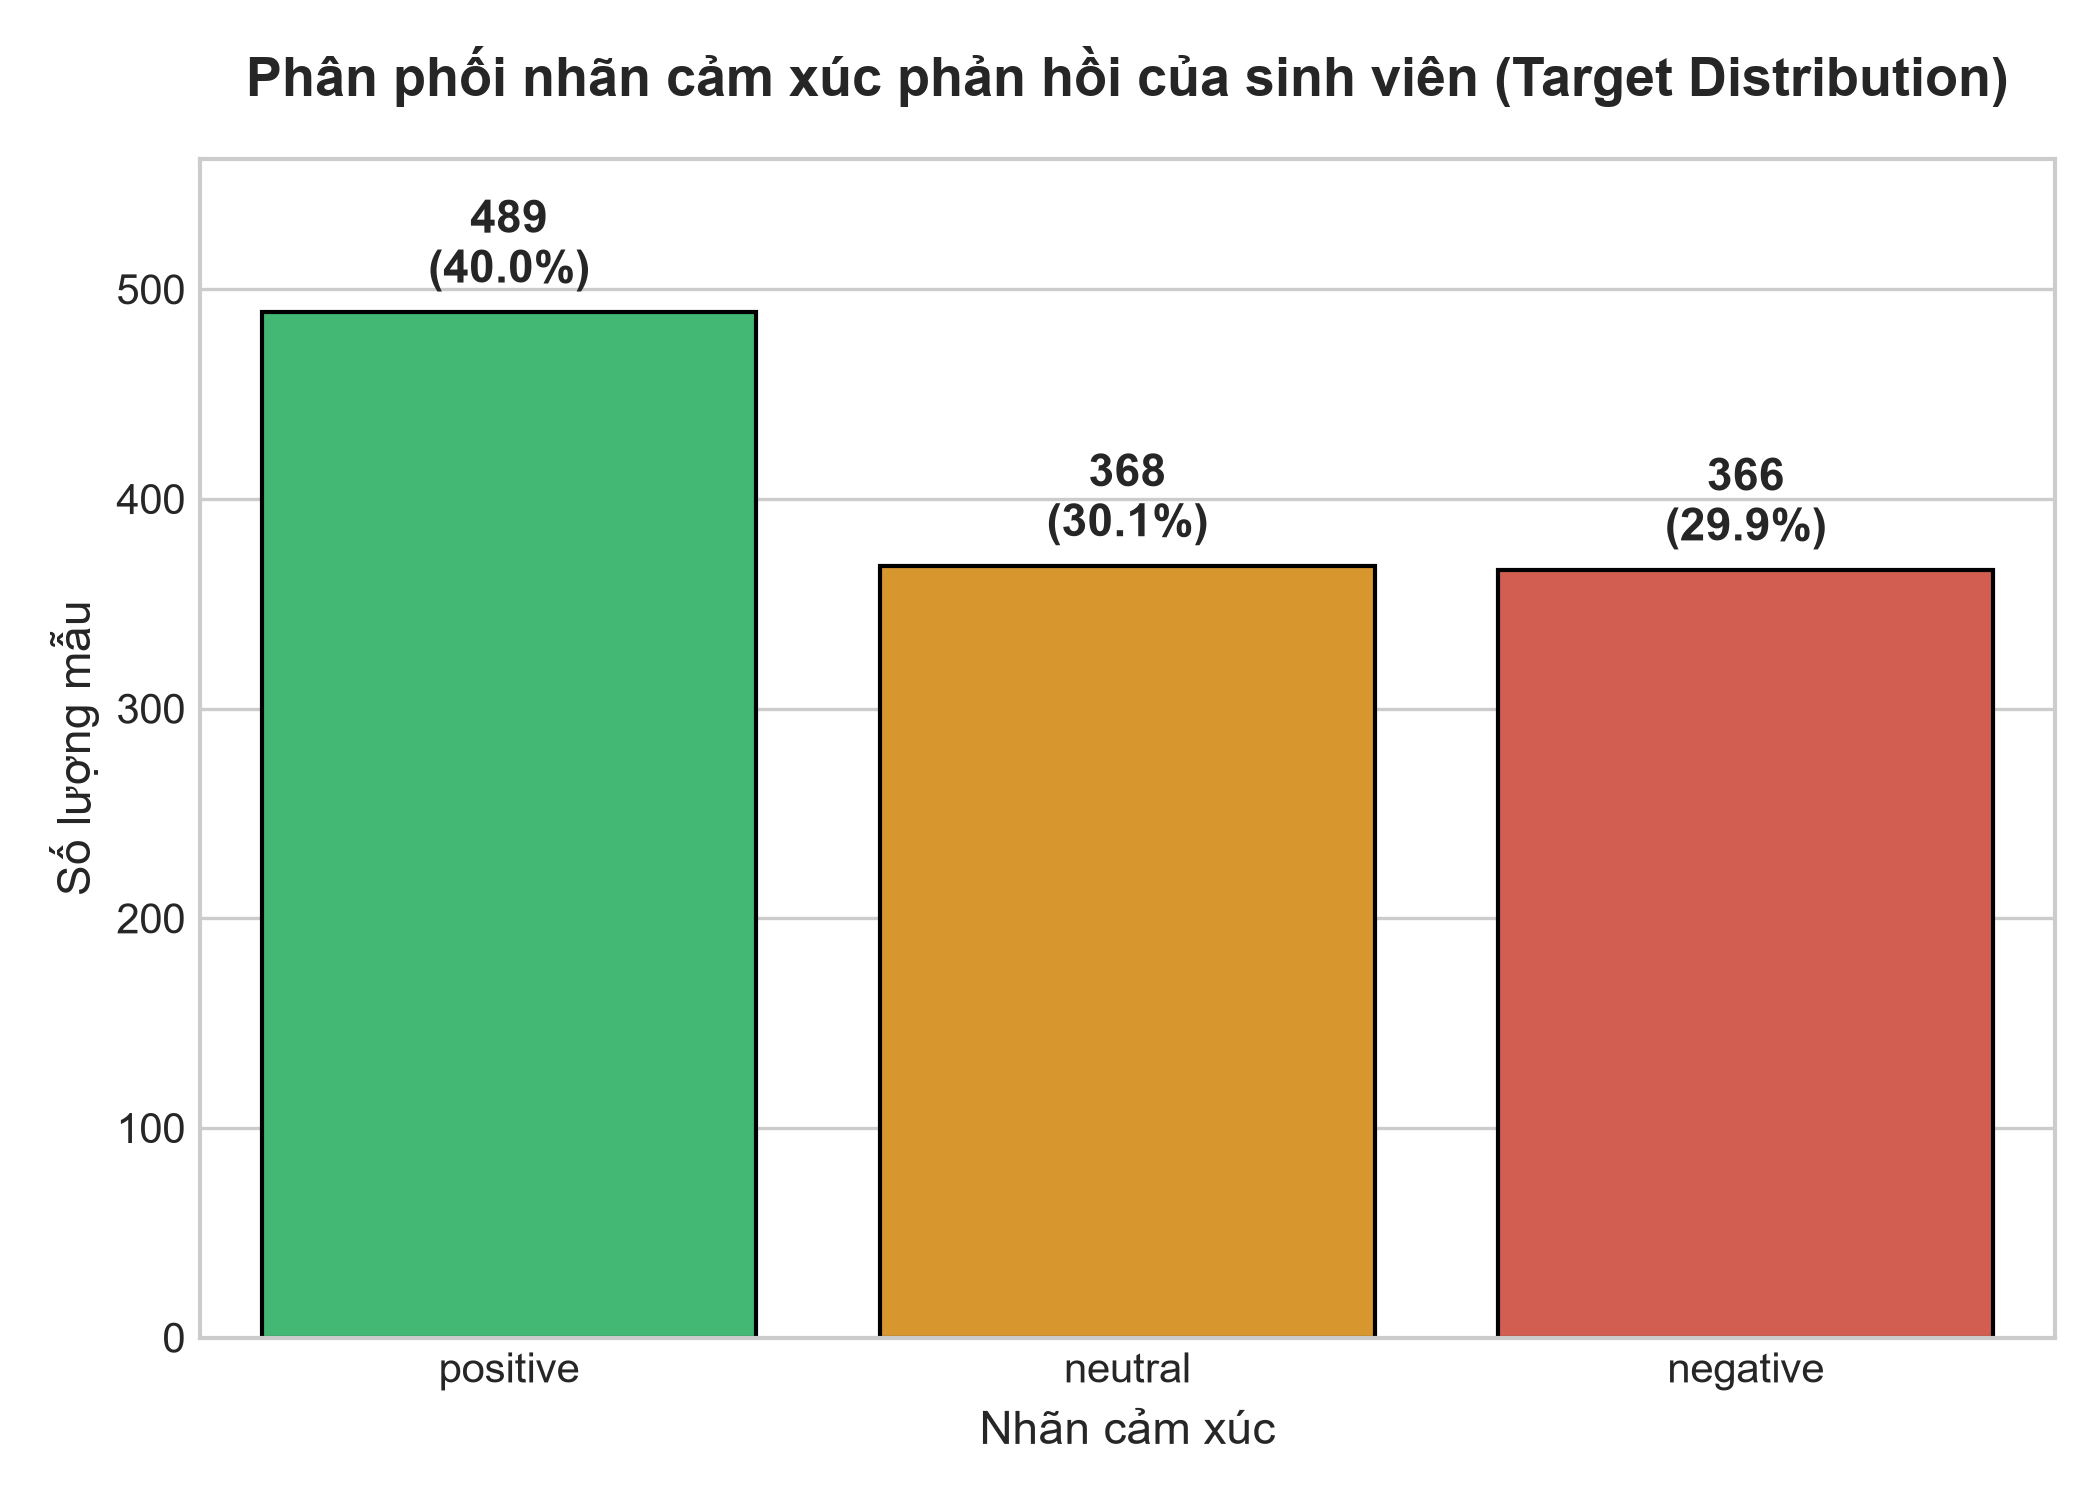
\includegraphics[width=0.65\textwidth]{../figures/class_distribution.png}
    \caption{Phân phối của nhãn cảm xúc mục tiêu trong tập dữ liệu.}
    \label{fig:class_dist}
\end{figure}

Qua kiểm tra định lượng, tập dữ liệu không có bất kỳ giá trị thiếu (missing values) nào và không có mẫu trùng lặp trong trường \texttt{feedback\_text}.
Phân phối nhãn mục tiêu (Hình \ref{fig:class_dist}) cho thấy sự chênh lệch nhẹ:
\begin{itemize}
    \item \textbf{Positive:} 489 mẫu (chiếm 39.98\%)
    \item \textbf{Neutral:} 368 mẫu (chiếm 30.09\%)
    \item \textbf{Negative:} 366 mẫu (chiếm 29.93\%)
\end{itemize}
Sự mất cân bằng nhẹ này khẳng định việc chỉ sử dụng độ đo \textbf{Accuracy} là không đầy đủ; báo cáo sẽ tập trung vào \textbf{Macro F1-Score} và \textbf{Confusion Matrix} để đánh giá công bằng trên cả 3 lớp.

\begin{figure}[H]
    \centering
    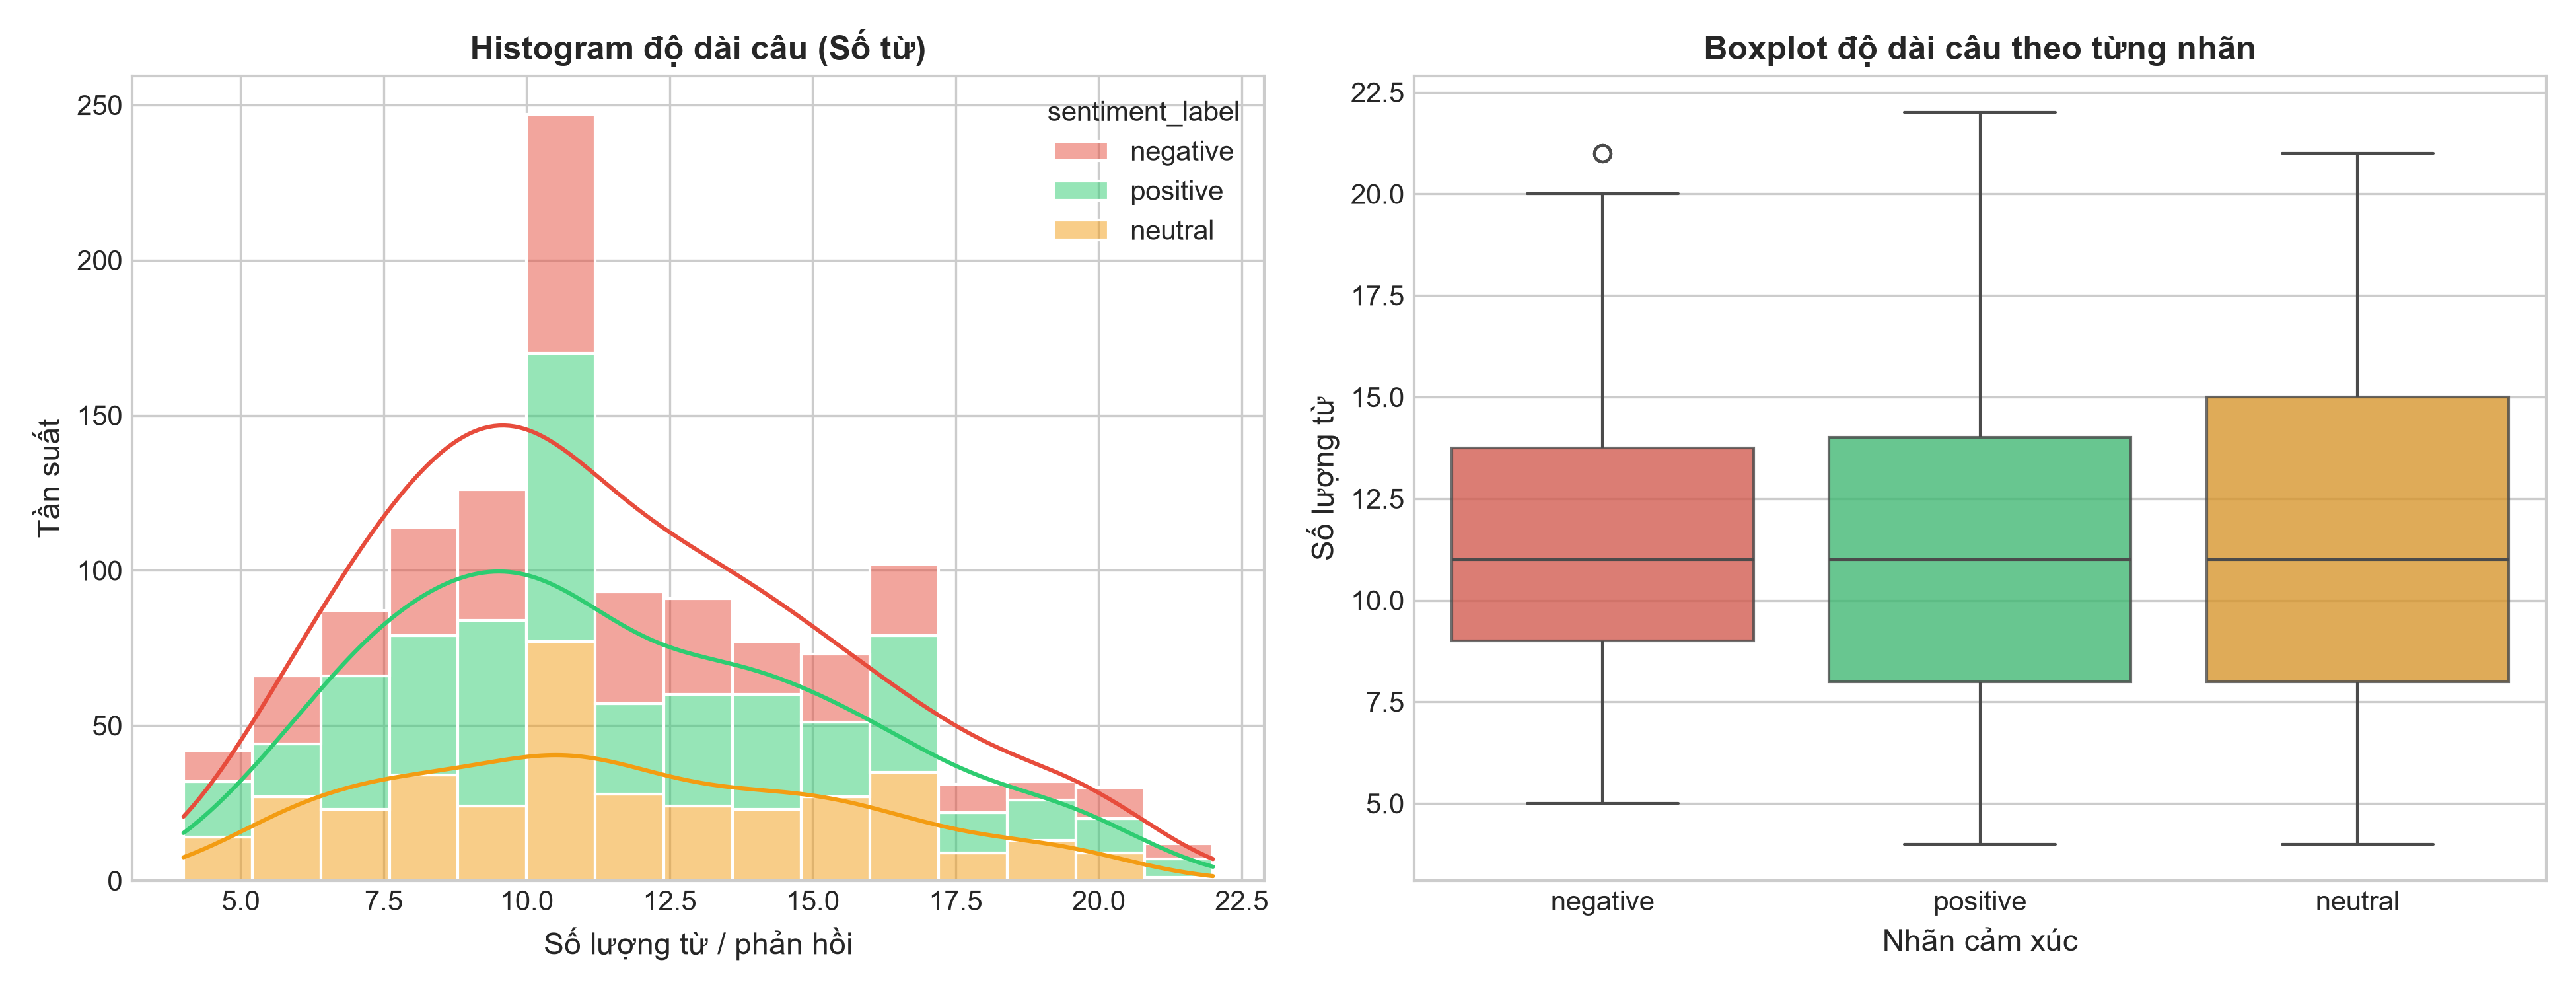
\includegraphics[width=0.85\textwidth]{../figures/text_length_distribution.png}
    \caption{Phân phối độ dài phản hồi (số lượng từ) theo từng nhóm cảm xúc.}
    \label{fig:length_dist}
\end{figure}

Hình \ref{fig:length_dist} thể hiện thống kê độ dài câu (tính theo số từ). Độ dài trung bình của các phản hồi là $11.45 \pm 3.9$ từ (ngắn nhất là 4 từ, dài nhất là 22 từ). Phân phối độ dài giữa 3 lớp cảm xúc là hoàn toàn tương đồng (trung bình Negative: 11.36, Neutral: 11.54, Positive: 11.46 từ). Điều này cho thấy độ dài câu không phải là đặc trưng phân biệt cảm xúc, mà tín hiệu cốt lõi nằm ở phân phối từ vựng ngữ nghĩa.

\begin{figure}[H]
    \centering
    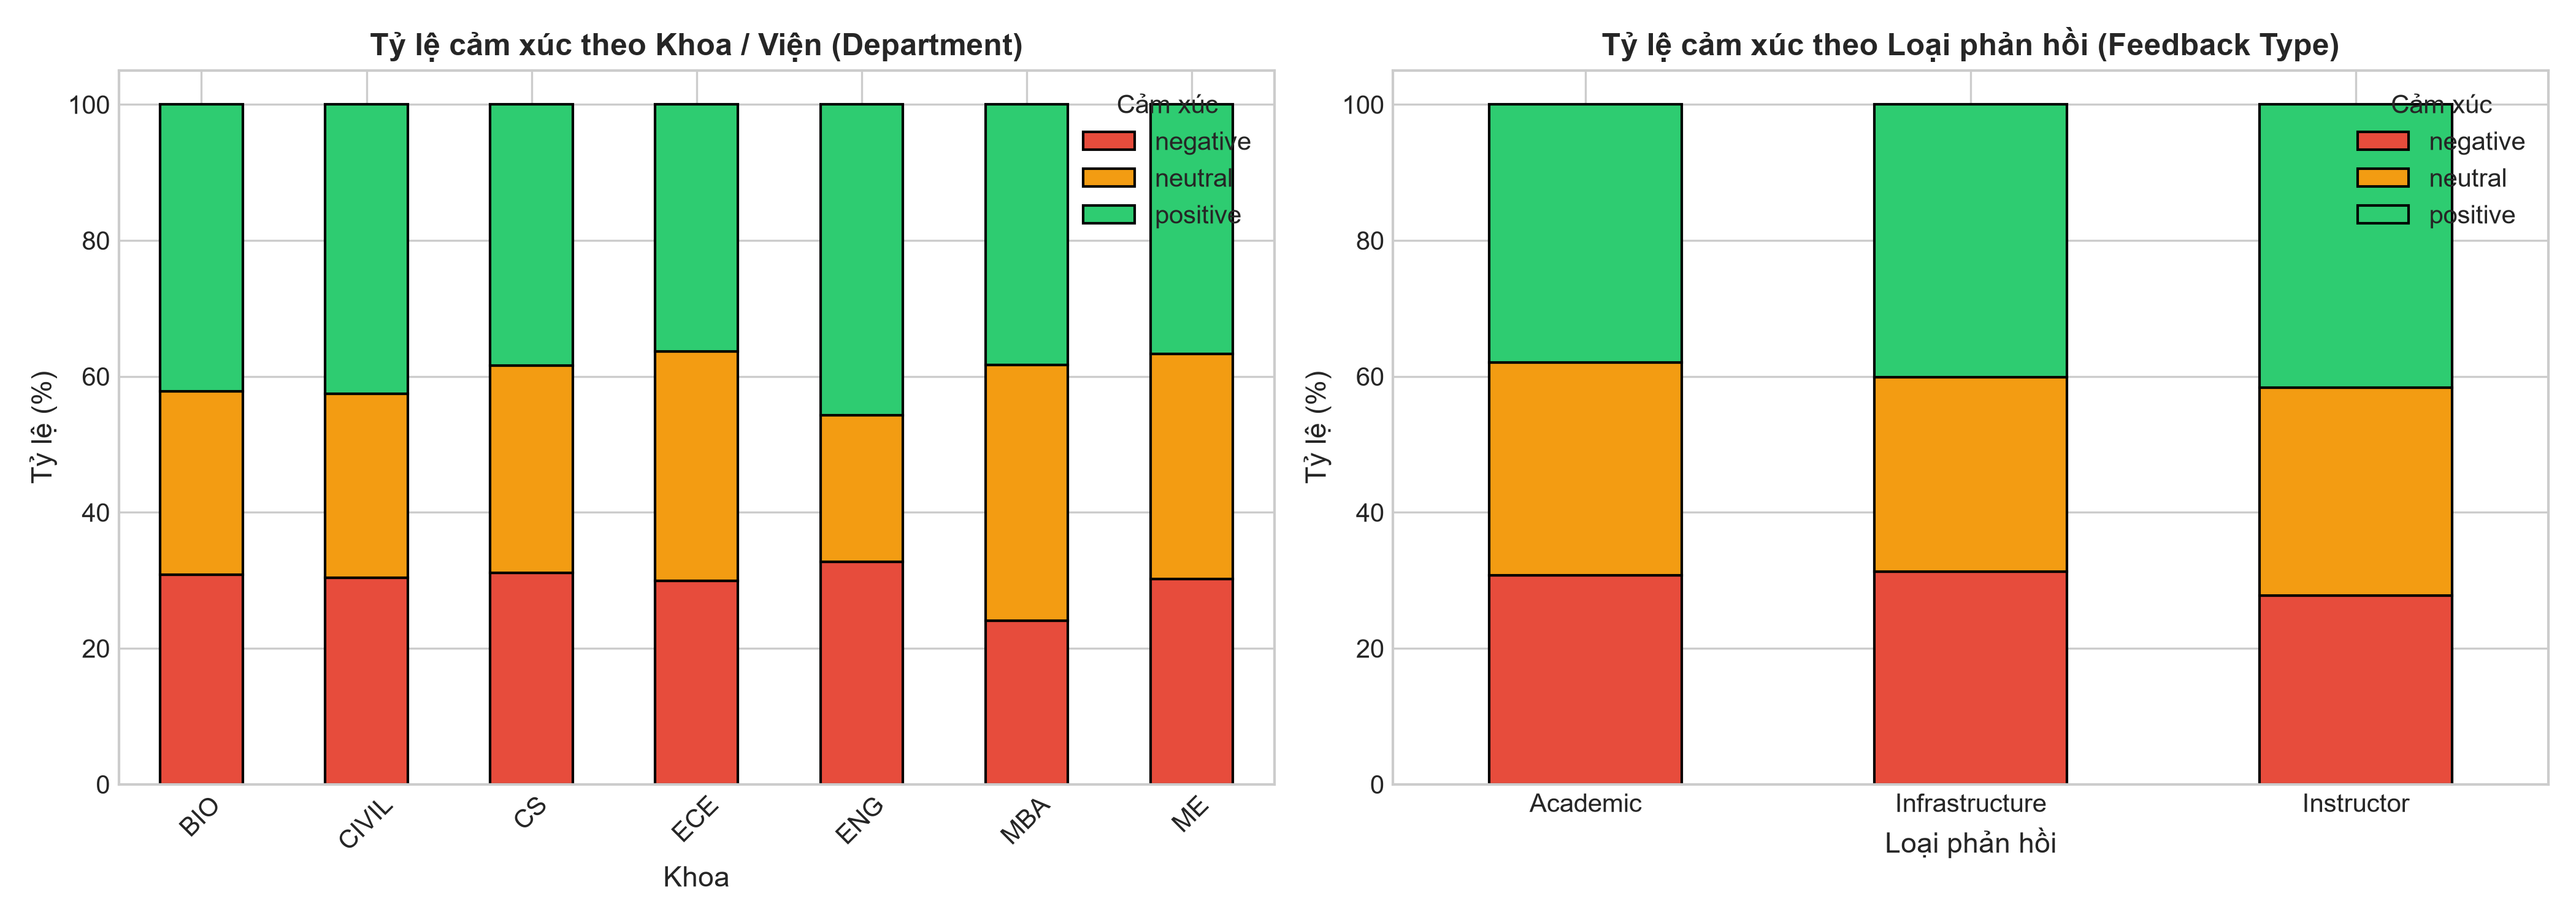
\includegraphics[width=0.88\textwidth]{../figures/department_feedback_sentiment.png}
    \caption{Tỷ lệ cảm xúc theo Khoa chuyên môn và Loại hình phản hồi.}
    \label{fig:dept_fb}
\end{figure}

Hình \ref{fig:dept_fb} mô tả tỷ lệ cảm xúc theo Khoa và Loại hình phản hồi. Các khoa kỹ thuật như CS, ECE, ME và các loại phản hồi về Giảng viên (Instructor) hoặc Cơ sở vật chất (Infrastructure) đều có tỷ lệ phản hồi tích cực chiếm khoảng 40\%, trong khi tiêu cực và trung tính chia đều khoảng 30\% mỗi loại.

\begin{figure}[H]
    \centering
    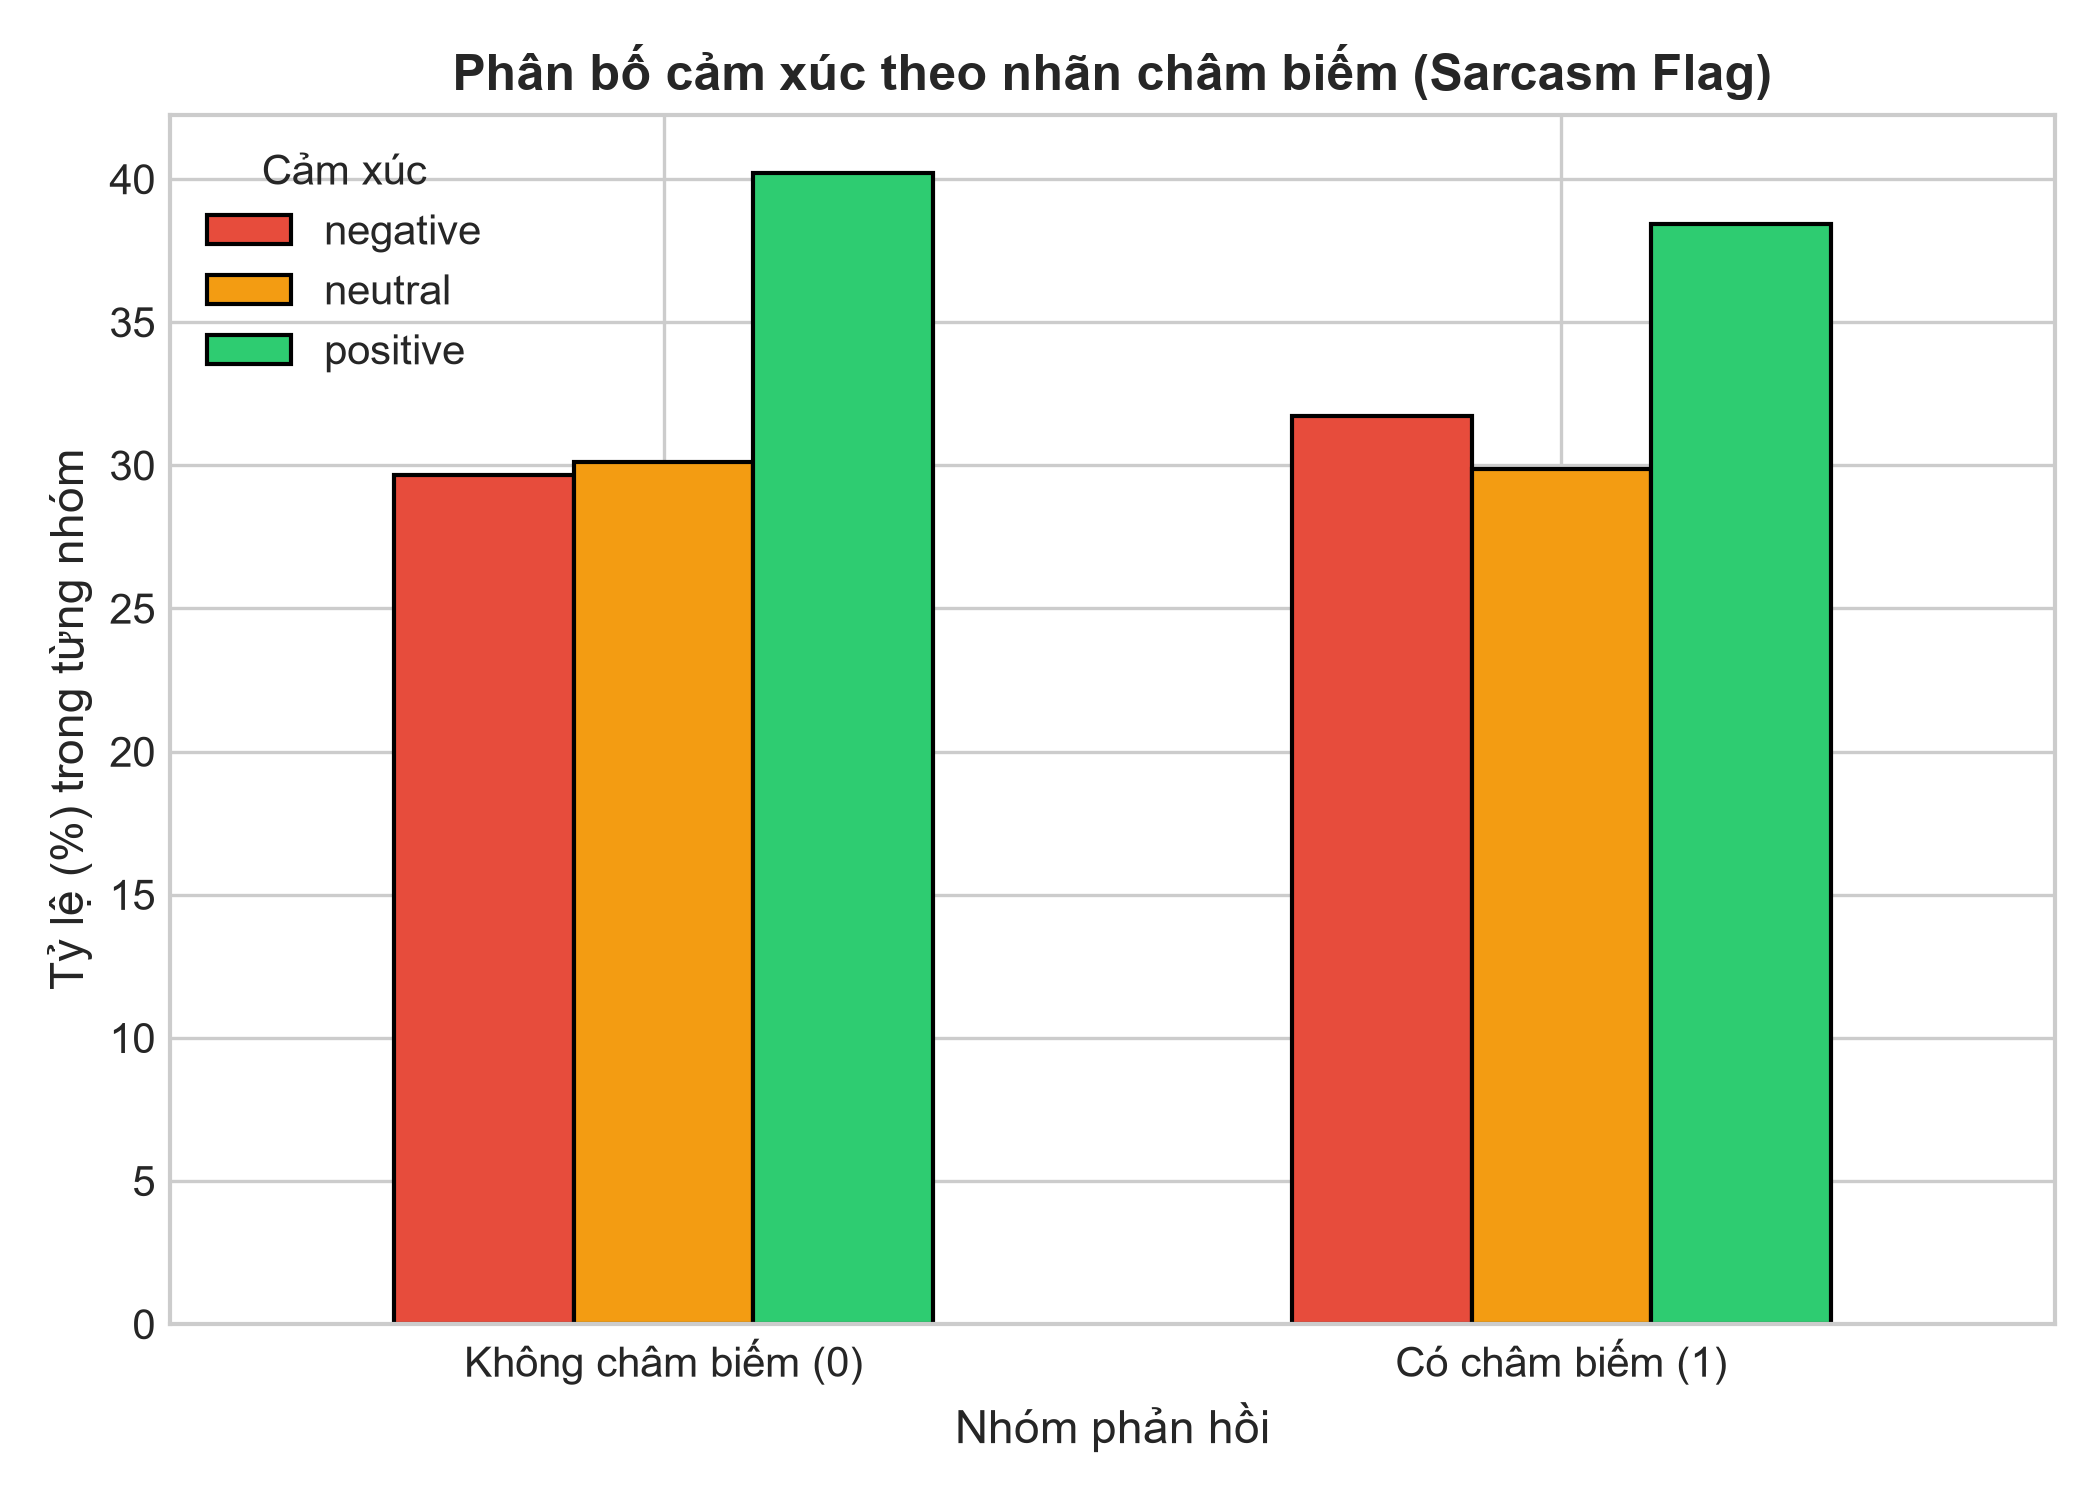
\includegraphics[width=0.58\textwidth]{../figures/sarcasm_impact.png}
    \caption{Phân bố cảm xúc theo cờ châm biếm (Sarcasm Flag).}
    \label{fig:sarcasm_eda}
\end{figure}

Một đặc điểm rất đáng chú ý trong tập dữ liệu là sự hiện diện của \textbf{164 mẫu châm biếm} (\texttt{sarcasm\_flag = 1}, chiếm 13.4\%). Hình \ref{fig:sarcasm_eda} cho thấy tỷ lệ cảm xúc ở nhóm châm biếm phân bổ tương đối đồng đều nhưng tạo ra nhiễu ngữ nghĩa nghiêm trọng cho các mô hình túi từ cổ điển (Bag-of-Words).

\begin{figure}[H]
    \centering
    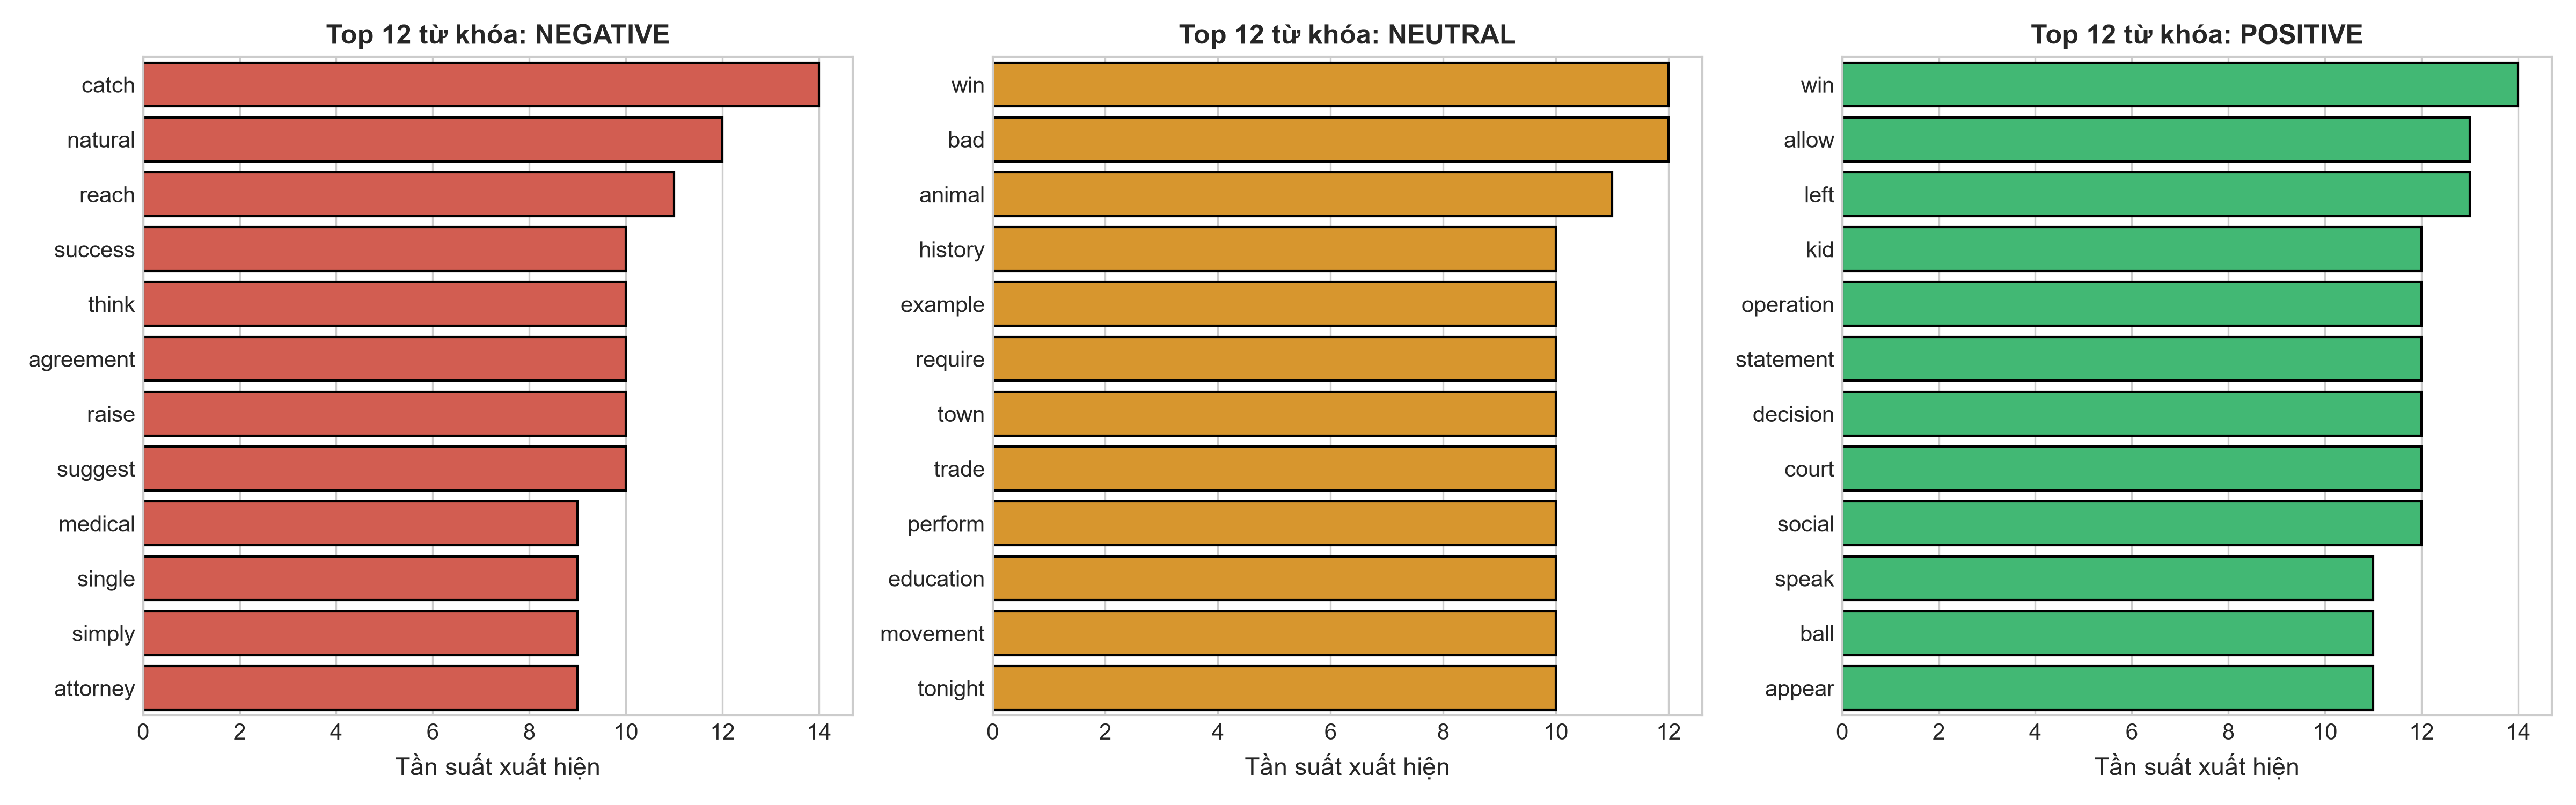
\includegraphics[width=0.95\textwidth]{../figures/top_words_per_sentiment.png}
    \caption{Top 12 từ khóa có tần suất xuất hiện cao nhất trong mỗi lớp cảm xúc.}
    \label{fig:top_words}
\end{figure}

Hình \ref{fig:top_words} trình bày các từ vựng xuất hiện nhiều nhất ở từng lớp sau khi lọc bỏ stopwords thông thường. Có thể nhận thấy sự giao thoa từ vựng lớn giữa các lớp (các từ như \textit{student, time, course, teacher, work} xuất hiện đồng thời ở cả ba nhóm), đặt ra thách thức lớn cho các thuật toán phân lớp.

\newpage
\section{Thiết kế giải pháp và quy trình học máy}

\subsection{Sơ đồ pipeline học máy tổng thể}
Quy trình xây dựng mô hình tuân thủ chặt chẽ mô hình chuẩn của bài toán Xử lý ngôn ngữ tự nhiên (NLP) được hướng dẫn trong học phần FIT4013:

\begin{center}
\fbox{Dữ liệu thô (CSV)} $\rightarrow$ \fbox{Tiền xử lý chuỗi} $\rightarrow$ \fbox{Train/Test Split (Stratified 80/20)} $\rightarrow$ \fbox{Fit Vectorizer (Train)} $\rightarrow$ \fbox{Transform (Train \& Test)} $\rightarrow$ \fbox{Huấn luyện \& Tinh chỉnh CV} $\rightarrow$ \fbox{Đánh giá Test Set \& Phân tích lỗi}
\end{center}

\subsection{Tiền xử lý dữ liệu và phòng chống Data Leakage}
Các bước tiền xử lý chuỗi văn bản được thực hiện gồm:
\begin{enumerate}
    \item \textbf{Chuyển chữ thường (Lowercasing):} Đưa toàn bộ ký tự về chữ thường nhằm đồng nhất các từ như "Good", "good", "GOOD".
    \item \textbf{Loại bỏ URL, thẻ HTML và ký tự đặc biệt:} Sử dụng Regular Expression để xóa bỏ các đường dẫn web, thẻ định dạng và các ký tự không thuộc bảng chữ cái tiếng Anh.
    \item \textbf{Chuẩn hóa khoảng trắng thừa:} Xóa bỏ các ký tự xuống dòng, tab và khoảng trắng liên tiếp.
    \item \textbf{Lọc Stopwords có kiểm soát:} Nếu loại bỏ stopwords một cách máy móc theo danh sách có sẵn của tiếng Anh, các từ phủ định như \textit{not, no, nor, never, neither, hardly, barely} sẽ bị xóa, làm triệt tiêu hoàn toàn sắc thái đảo ngược cảm xúc (ví dụ: "not good" bị biến thành "good"). Do đó, nhóm xây dựng danh sách \texttt{CUSTOM\_STOP\_WORDS} bằng cách giữ lại các từ phủ định cốt lõi.
\end{enumerate}

\textbf{Quy trình phân chia dữ liệu chống rò rỉ (Data Leakage):}
Để ngăn chặn hoàn toàn hiện tượng rò rỉ thông tin từ tập kiểm thử vào quá trình học:
\begin{itemize}
    \item Dữ liệu được phân chia thành tập huấn luyện \textbf{Train (80\% - 978 mẫu)} và tập kiểm thử \textbf{Test (20\% - 245 mẫu)}.
    \item Sử dụng kỹ thuật phân tầng (\texttt{stratify=y}) để bảo đảm tỷ lệ giữa các nhãn \texttt{positive}, \texttt{neutral}, \texttt{negative} ở cả hai tập là hoàn toàn đồng nhất ($40\% - 30\% - 30\%$).
    \item Cố định giá trị \texttt{random\_state = 42} giúp mọi kết quả có tính tái lập (reproducibility) tuyệt đối.
    \item \textbf{Nguyên tắc cốt lõi:} Bộ chuyển đổi vector hóa (\texttt{CountVectorizer}, \texttt{TfidfVectorizer}) chỉ được phép gọi phương thức \texttt{fit()} trên tập Train, sau đó áp dụng \texttt{transform()} trên tập Test.
\end{itemize}

\subsection{Biểu diễn và trích xuất đặc trưng (Feature Representation)}
Báo cáo tiến hành thử nghiệm và so sánh hai phương pháp trích xuất đặc trưng kinh điển:
\begin{enumerate}
    \item \textbf{Bag-of-Words (CountVectorizer):}
    Biểu diễn văn bản dưới dạng vector tần số xuất hiện của các từ trong từ điển:
    \begin{equation}
        \mathbf{x} = [c_1, c_2, \dots, c_V]^T
    \end{equation}
    trong đó $c_i$ là số lần xuất hiện của từ thứ $i$ trong câu, $V$ là kích thước từ vựng.
    
    \item \textbf{TF-IDF (Term Frequency - Inverse Document Frequency):}
    Cân chỉnh trọng số của từng từ bằng cách phạt những từ xuất hiện quá phổ biến ở mọi tài liệu và đề cao những từ mang tính đặc trưng:
    \begin{equation}
        \text{TF-IDF}(t, d, D) = \text{TF}(t, d) \times \text{IDF}(t, D)
    \end{equation}
    với:
    \begin{equation}
        \text{TF}(t, d) = \frac{f_{t, d}}{\sum_{t' \in d} f_{t', d}}, \quad \text{IDF}(t, D) = \ln \left( \frac{1 + |D|}{1 + |\{d \in D : t \in d\}|} \right) + 1
    \end{equation}
\end{enumerate}

Nhóm thiết kế 6 cấu hình đặc trưng bao gồm: BoW Unigram, BoW Unigram+Bigram, TF-IDF Unigram, TF-IDF Unigram+Bigram, TF-IDF với $min\_df=2$, và TF-IDF với sublinear scaling ($1 + \log(TF)$).

\subsection{Mô hình học máy và cơ sở lý thuyết}

Trong phạm vi các thuật toán đã học trong học phần (K-NN, Naive Bayes, Cây quyết định và K-means), nhóm lựa chọn các thuật toán học có giám sát phù hợp nhất cho bài toán phân loại đa lớp:

\subsubsection{1. Mô hình Baseline: Dummy Classifier (Majority Class)}
Mô hình luôn dự đoán lớp chiếm đa số (\texttt{positive}). Mục tiêu là tạo ra mốc chuẩn tối thiểu (benchmark baseline) để chứng minh tính hiệu quả của các mô hình học máy thực sự.

\subsubsection{2. Mô hình cốt lõi: Multinomial Naive Bayes (MNB)}
Multinomial Naive Bayes là mô hình chuẩn mực được thiết kế đặc thù cho bài toán phân loại văn bản với đặc trưng đếm và TF-IDF. Dựa trên Định lý Bayes và giả định độc lập có điều kiện giữa các từ:
\begin{equation}
    P(c \mid \mathbf{x}) \propto P(c) \prod_{i=1}^{V} P(w_i \mid c)^{x_i}
\end{equation}
Xác suất có điều kiện của từ $w_i$ với kỹ thuật làm trơn Laplace (Laplace smoothing) được tính bởi:
\begin{equation}
    P(w_i \mid c) = \frac{N_{ci} + \alpha}{N_c + \alpha V}
\end{equation}
trong đó $N_{ci}$ là tổng số lần từ $w_i$ xuất hiện trong lớp $c$, $N_c$ là tổng số từ của lớp $c$, và $\alpha > 0$ là siêu tham số làm trơn (smoothing parameter) cần tinh chỉnh.

\subsubsection{3. Mô hình so sánh 1: Cây quyết định (Decision Tree Classifier)}
Cây quyết định phân chia không gian đặc trưng bằng cách tối đa hóa mức giảm độ hỗn loạn (impurity) tại mỗi nút phân nhánh. Hai tiêu chí đo độ tinh khiết được đưa vào thử nghiệm:
\begin{itemize}
    \item Chỉ số Gini (Gini Impurity):
    \begin{equation}
        I_G(p) = 1 - \sum_{k=1}^{C} p_k^2
    \end{equation}
    \item Độ hỗn loạn Entropy (Information Gain):
    \begin{equation}
        H(p) = -\sum_{k=1}^{C} p_k \log_2(p_k)
    \end{equation}
\end{itemize}
Siêu tham số tinh chỉnh gồm: \texttt{criterion} $\in \{\text{'gini'}, \text{'entropy'}\}$, \texttt{max\_depth} $\in \{5, 10, 15, 20, \text{None}\}$, và \texttt{min\_samples\_split}.

\subsubsection{4. Mô hình so sánh 2: K-Láng giềng gần nhất (K-Nearest Neighbors - KNN)}
K-NN là thuật toán học lười (lazy learning) phi tham số. Với mỗi mẫu kiểm thử, mô hình tìm $K$ mẫu huấn luyện gần nhất dựa trên khoảng cách. Với dữ liệu văn bản sau khi chuẩn hóa độ dài vector, khoảng cách Cosine thường vượt trội hơn khoảng cách Euclidean:
\begin{equation}
    d_{\text{Cosine}}(\mathbf{u}, \mathbf{v}) = 1 - \frac{\mathbf{u} \cdot \mathbf{v}}{\|\mathbf{u}\|_2 \|\mathbf{v}\|_2}
\end{equation}
Siêu tham số tinh chỉnh gồm: $k \in \{3, 5, 7, 9, 11, 15\}$, độ đo khoảng cách \texttt{metric} $\in \{\text{'cosine'}, \text{'euclidean'}\}$, và trọng số láng giềng \texttt{weights} $\in \{\text{'uniform'}, \text{'distance'}\}$.

\newpage
\section{Phân tích mã nguồn và chức năng}

\subsection{Cấu trúc chương trình}
Mã nguồn được tổ chức theo chuẩn kiến trúc module học máy chuyên nghiệp:
\begin{itemize}
    \item \texttt{src/eda.py}: Tải dữ liệu, tính toán các chỉ số thống kê mô tả độ dài, phân tích tương quan giữa các nhãn và lưu các biểu đồ vào thư mục \texttt{figures/}.
    \item \texttt{src/preprocessing.py}: Chứa hàm \texttt{clean\_text} thực hiện chuẩn hóa văn bản, xóa ký tự đặc biệt, lọc stop words bảo lưu từ phủ định.
    \item \texttt{src/features.py}: Cung cấp hàm \texttt{get\_vectorizer} và \texttt{build\_vectorizer\_configurations} khởi tạo các pipeline CountVectorizer và TfidfVectorizer.
    \item \texttt{src/models.py}: Định nghĩa các mô hình Baseline, MNB, Decision Tree, KNN và không gian tham số cho \texttt{GridSearchCV}.
    \item \texttt{src/evaluate.py}: Tính toán các độ đo \texttt{compute\_metrics}, vẽ heatmap ma trận nhầm lẫn và module phân tích lỗi \texttt{analyze\_errors}.
    \item \texttt{main.py}: Tích hợp toàn bộ quy trình đầu-cuối từ nạp dữ liệu đến huấn luyện, xuất biểu đồ và lưu trữ mô hình ra thư mục \texttt{models/}.
    \item \texttt{app.py}: Ứng dụng web trực quan xây dựng trên thư viện Streamlit (phục vụ mục Điểm thưởng).
\end{itemize}

\subsection{Các đoạn mã nguồn quan trọng}

\subsubsection{Xử lý văn bản bảo lưu từ phủ định}
\begin{lstlisting}[language=Python, caption=Hàm tiền xử lý chuỗi và bảo lưu từ phủ định]
NEGATION_WORDS = {'not', 'no', 'nor', 'never', 'neither', 'hardly', 'barely'}
CUSTOM_STOP_WORDS = set(ENGLISH_STOP_WORDS) - NEGATION_WORDS

def clean_text(text: str, remove_stopwords: bool = True) -> str:
    if not isinstance(text, str):
        return ""
    text = text.lower()
    text = re.sub(r'https?://\S+|www\.\S+', ' ', text)
    text = re.sub(r'[' + re.escape(string.punctuation) + r']', ' ', text)
    text = re.sub(r'[^a-zA-Z\s]', ' ', text)
    words = text.split()
    if remove_stopwords:
        words = [w for w in words if w not in CUSTOM_STOP_WORDS and len(w) > 1]
    return " ".join(words)
\end{lstlisting}

\subsubsection{Tìm kiếm siêu tham số bằng 5-fold Stratified CV}
\begin{lstlisting}[language=Python, caption=Quy trình tối ưu hóa siêu tham số bằng GridSearchCV]
skf = StratifiedKFold(n_splits=5, shuffle=True, random_state=42)

# Tinh chinh Multinomial Naive Bayes
param_nb = {"alpha": [0.01, 0.05, 0.1, 0.5, 1.0, 2.0]}
gs_nb = GridSearchCV(MultinomialNB(), param_nb, cv=skf, scoring="f1_macro", n_jobs=-1)
gs_nb.fit(X_train_vec, y_train)
best_nb = gs_nb.best_estimator_

# Tinh chinh Decision Tree
param_dt = {
    "criterion": ["gini", "entropy"],
    "max_depth": [5, 10, 15, 20, None],
    "min_samples_split": [2, 5, 10]
}
gs_dt = GridSearchCV(DecisionTreeClassifier(random_state=42), param_dt, cv=skf, scoring="f1_macro", n_jobs=-1)
gs_dt.fit(X_train_vec, y_train)
best_dt = gs_dt.best_estimator_
\end{lstlisting}

\newpage
\section{Thử nghiệm và kết quả}

\subsection{Thiết lập thí nghiệm}
\begin{itemize}
    \item \textbf{Phân chia tập dữ liệu:} 80\% Train ($978$ mẫu) và 20\% Test ($245$ mẫu), Stratified theo nhãn cảm xúc, cố định \texttt{random\_state = 42}.
    \item \textbf{Đánh giá chéo:} 5-fold Stratified Cross-Validation trên tập Train để lựa chọn siêu tham số tối ưu theo tiêu chí \texttt{f1\_macro}.
    \item \textbf{Tập kiểm thử độc lập:} Toàn bộ bảng kết quả và ma trận nhầm lẫn được tính toán trên 245 mẫu Test chưa từng xuất hiện trong quá trình huấn luyện hay tinh chỉnh.
    \item \textbf{Tiêu chí đánh giá:} Accuracy, Macro Precision, Macro Recall, Macro F1, Weighted F1 và Confusion Matrix.
\end{itemize}

\subsection{So sánh các phương pháp biểu diễn đặc trưng}
Bảng \ref{tab:vec_results} và Hình \ref{fig:vec_comp} trình bày kết quả thử nghiệm trên mô hình Multinomial Naive Bayes ($\alpha=1.0$) với các kỹ thuật biểu diễn đặc trưng khác nhau.

\begin{table}[H]
\centering
\caption{So sánh ảnh hưởng của phương pháp biểu diễn đặc trưng tới MultinomialNB}
\label{tab:vec_results}
\begin{tabular}{lcccc}
\toprule
\textbf{Phương pháp biểu diễn} & \textbf{Số lượng từ vựng} & \textbf{Accuracy} & \textbf{Macro F1} & \textbf{Weighted F1} \\
\midrule
BoW (Unigram) & 767 & 0.3918 & \textbf{0.3780} & 0.3888 \\
BoW (Unigram + Bigram) & 8,601 & 0.3918 & 0.3409 & 0.3635 \\
TF-IDF (Unigram) & 767 & \textbf{0.4000} & 0.3605 & 0.3739 \\
TF-IDF (Unigram + Bigram) & 8,601 & 0.3959 & 0.2545 & 0.2846 \\
TF-IDF ($min\_df=2$) & 767 & \textbf{0.4000} & 0.3605 & 0.3739 \\
TF-IDF (Sublinear TF) & 767 & \textbf{0.4000} & 0.3608 & 0.3742 \\
\bottomrule
\end{tabular}
\end{table}

\begin{figure}[H]
    \centering
    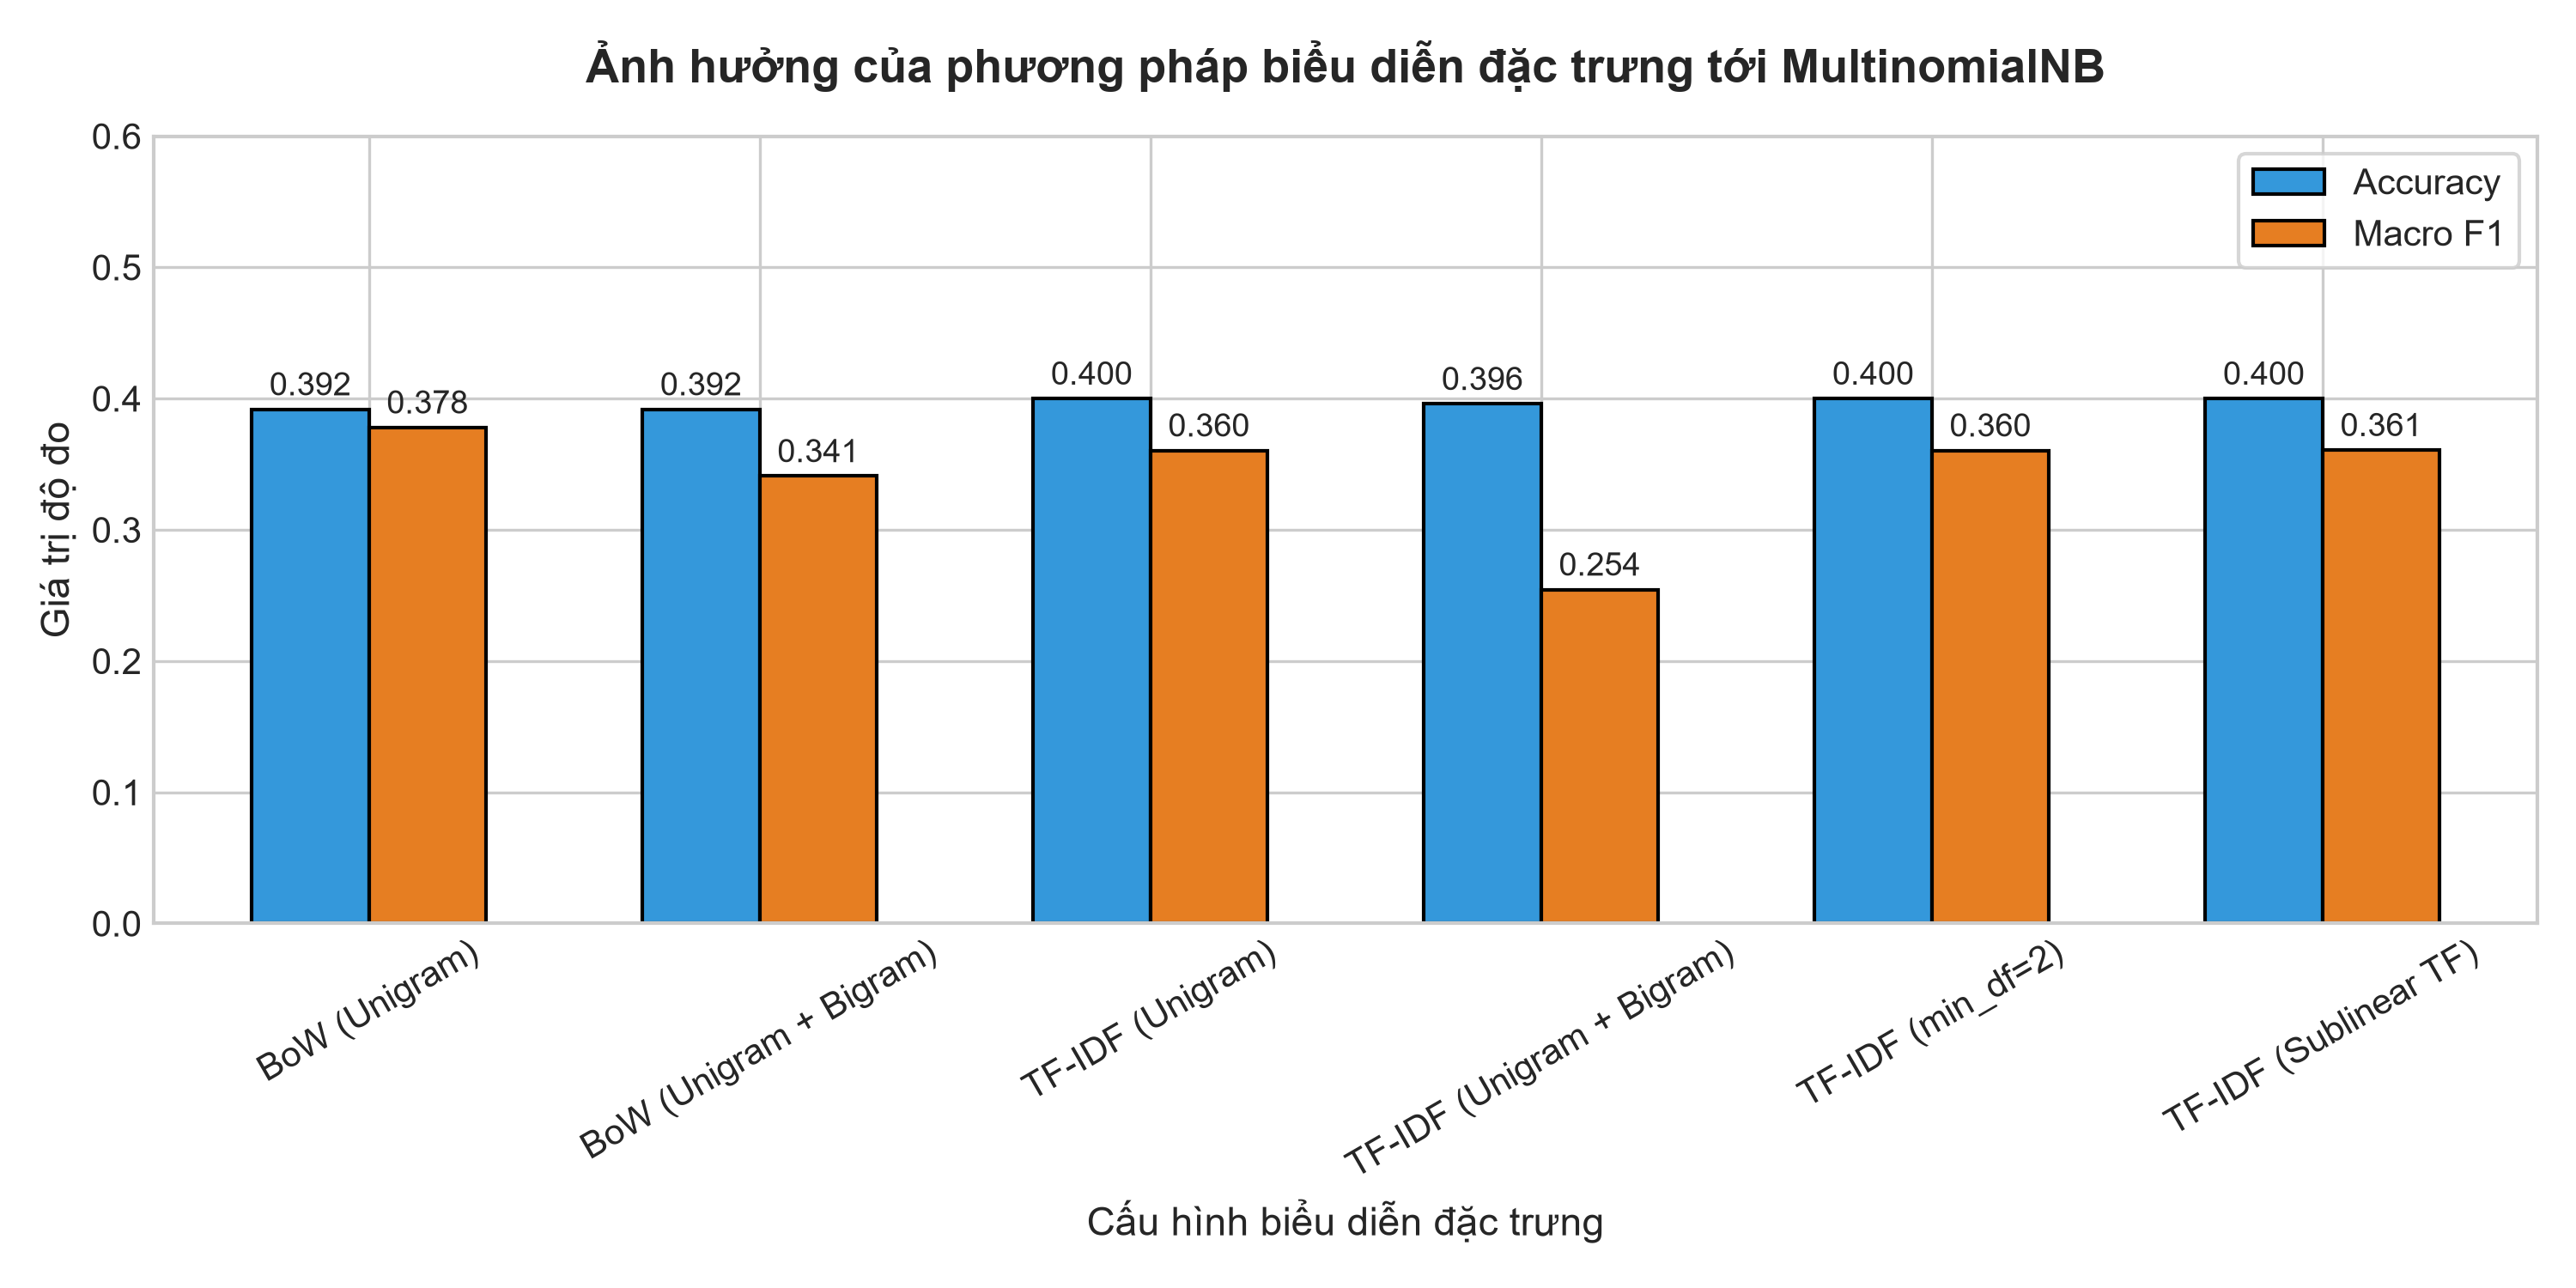
\includegraphics[width=0.85\textwidth]{../figures/vectorizer_comparison.png}
    \caption{Biểu đồ so sánh Accuracy và Macro-F1 giữa các cấu hình biểu diễn đặc trưng.}
    \label{fig:vec_comp}
\end{figure}

\subsection{Bảng tổng hợp kết quả giữa các mô hình}
Sau khi tìm kiếm siêu tham số tối ưu bằng 5-fold CV, các mô hình tốt nhất được đánh giá trên tập Test (Bảng \ref{tab:model_results} và Hình \ref{fig:model_comp}).

\begin{table}[H]
\centering
\caption{Bảng kết quả so sánh hiệu năng các mô hình trên tập kiểm thử (Test Set)}
\label{tab:model_results}
\begin{tabular}{lccccc}
\toprule
\textbf{Mô hình} & \textbf{Siêu tham số tối ưu} & \textbf{Accuracy} & \textbf{Macro Prec} & \textbf{Macro Rec} & \textbf{Macro F1} \\
\midrule
\textbf{Baseline (Majority)} & Most Frequent (Positive) & 0.4000 & 0.1333 & 0.3333 & 0.1905 \\
\textbf{Multinomial Naive Bayes} & $\alpha = 0.5$ & 0.3878 & \textbf{0.3693} & \textbf{0.3648} & \textbf{0.3570} \\
\textbf{Decision Tree} & \texttt{entropy}, \texttt{depth=None} & 0.3429 & 0.3362 & 0.3356 & 0.3357 \\
\textbf{K-Nearest Neighbors} & $k=9$, \texttt{cosine}, \texttt{distance} & 0.3265 & 0.3159 & 0.3182 & 0.3154 \\
\bottomrule
\end{tabular}
\end{table}

\begin{figure}[H]
    \centering
    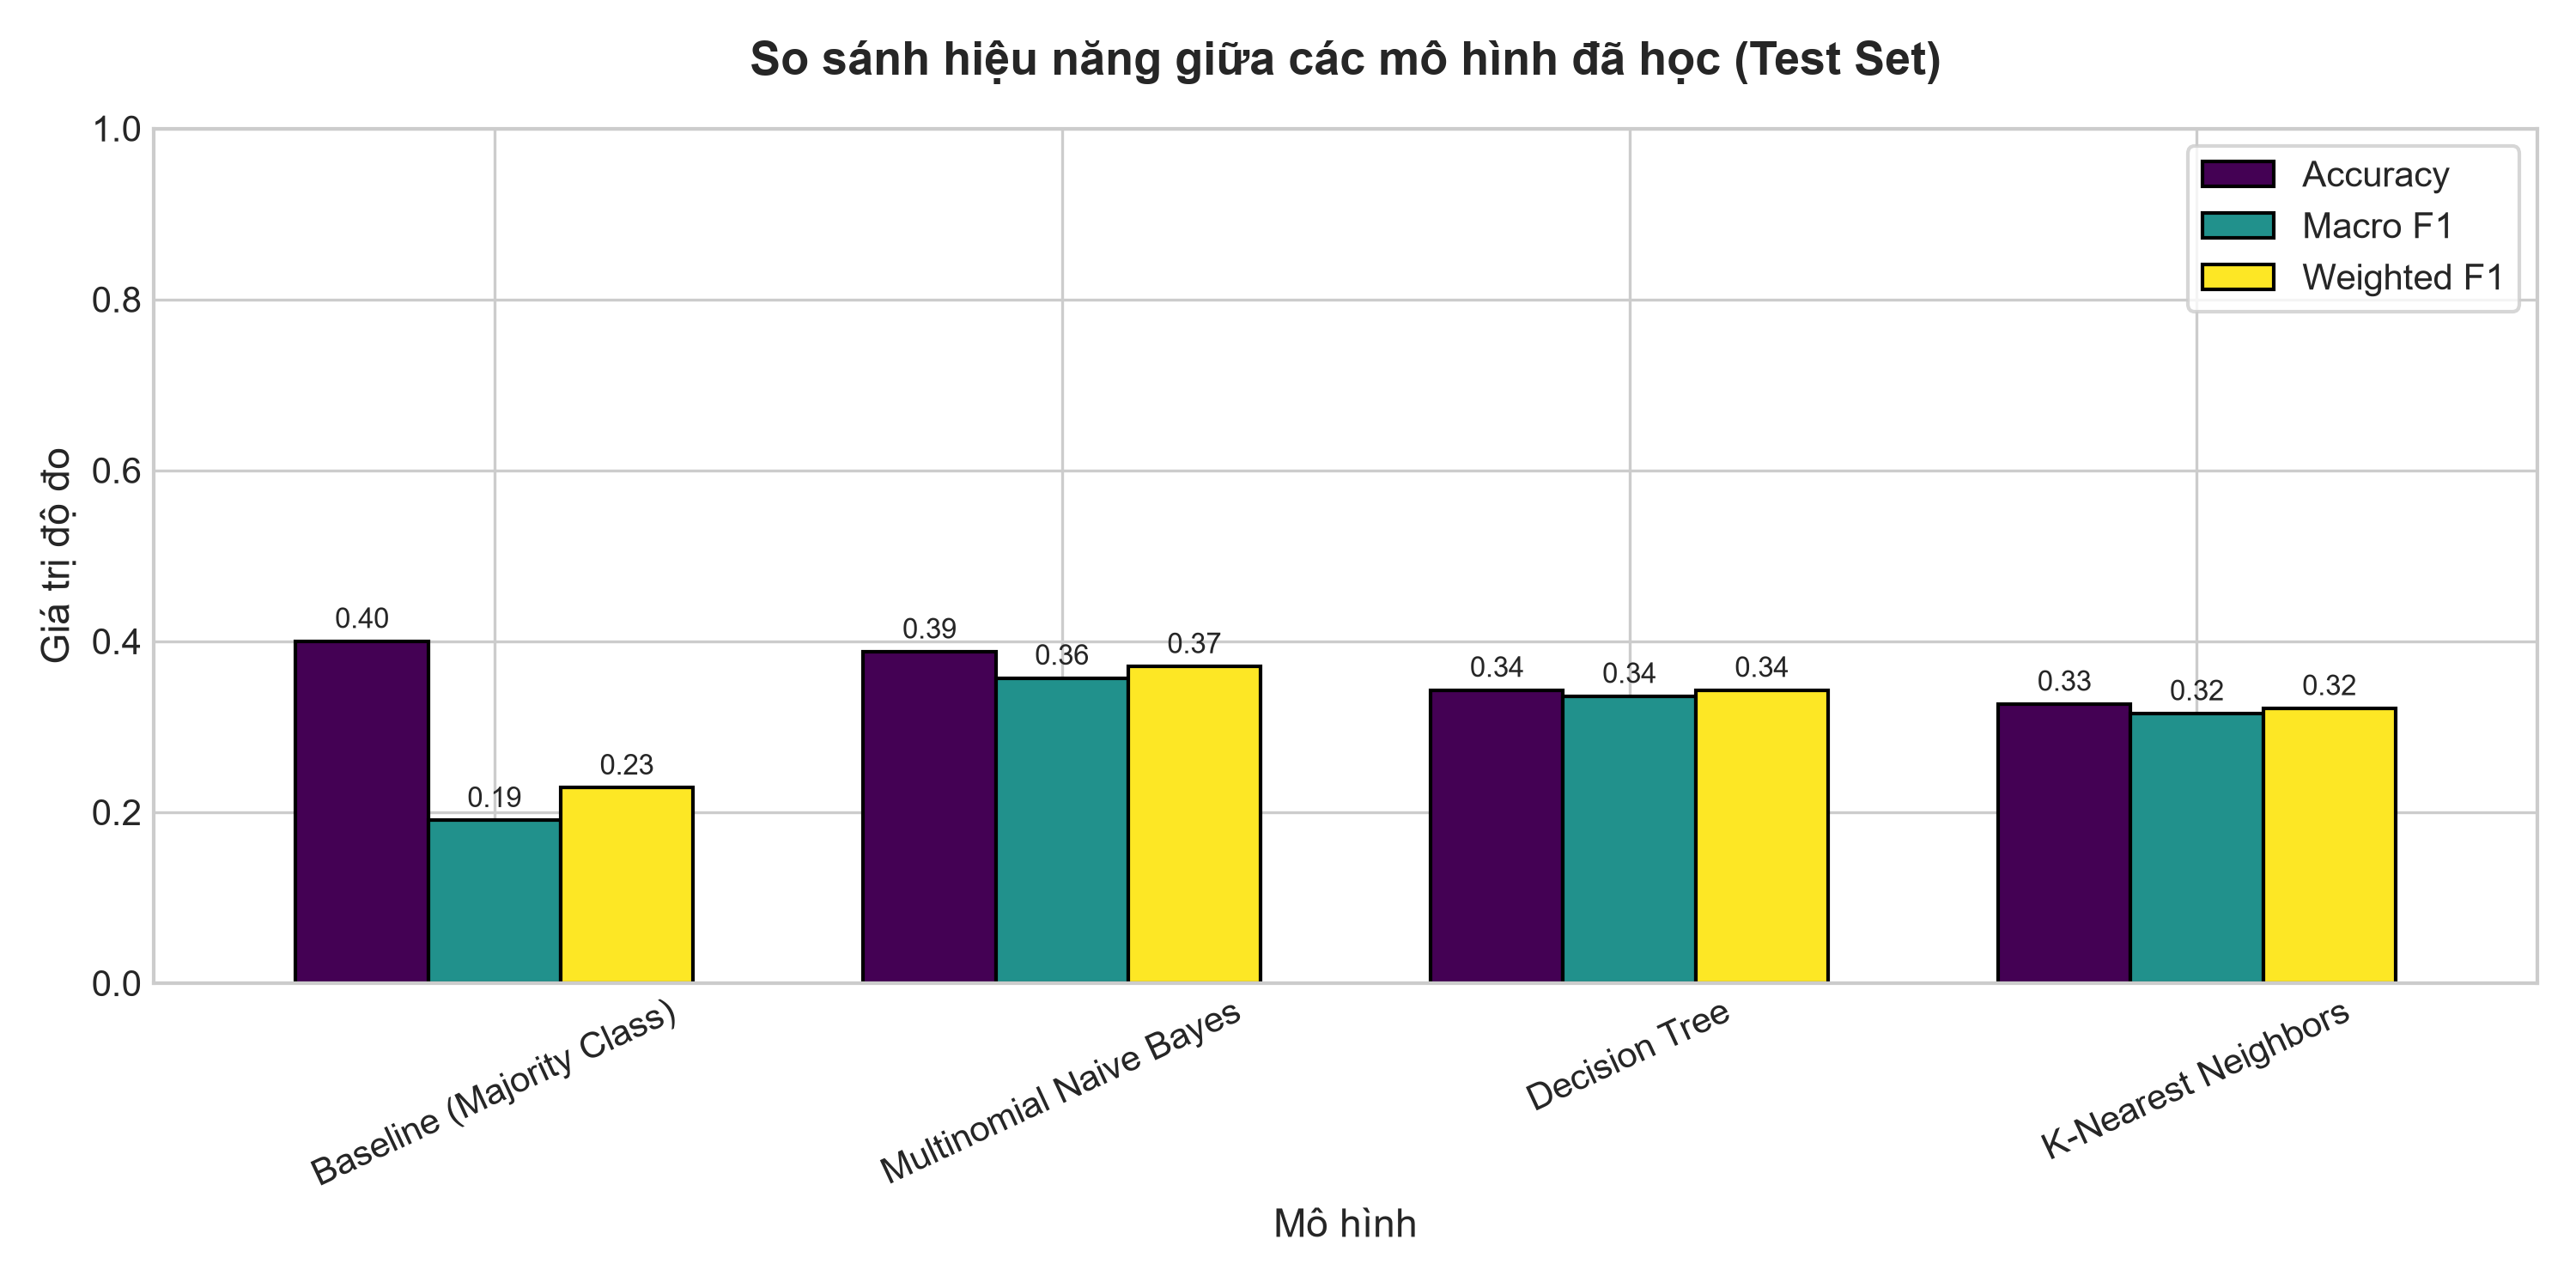
\includegraphics[width=0.88\textwidth]{../figures/model_comparison_metrics.png}
    \caption{So sánh trực quan các chỉ số Accuracy, Macro-F1 và Weighted-F1 giữa các mô hình.}
    \label{fig:model_comp}
\end{figure}

\subsection{Trực quan hóa ma trận nhầm lẫn (Confusion Matrices)}
Hình \ref{fig:cms} hiển thị ma trận nhầm lẫn chi tiết của cả 4 phương án thử nghiệm trên tập kiểm thử.

\begin{figure}[H]
    \centering
    \begin{subfigure}[b]{0.48\textwidth}
        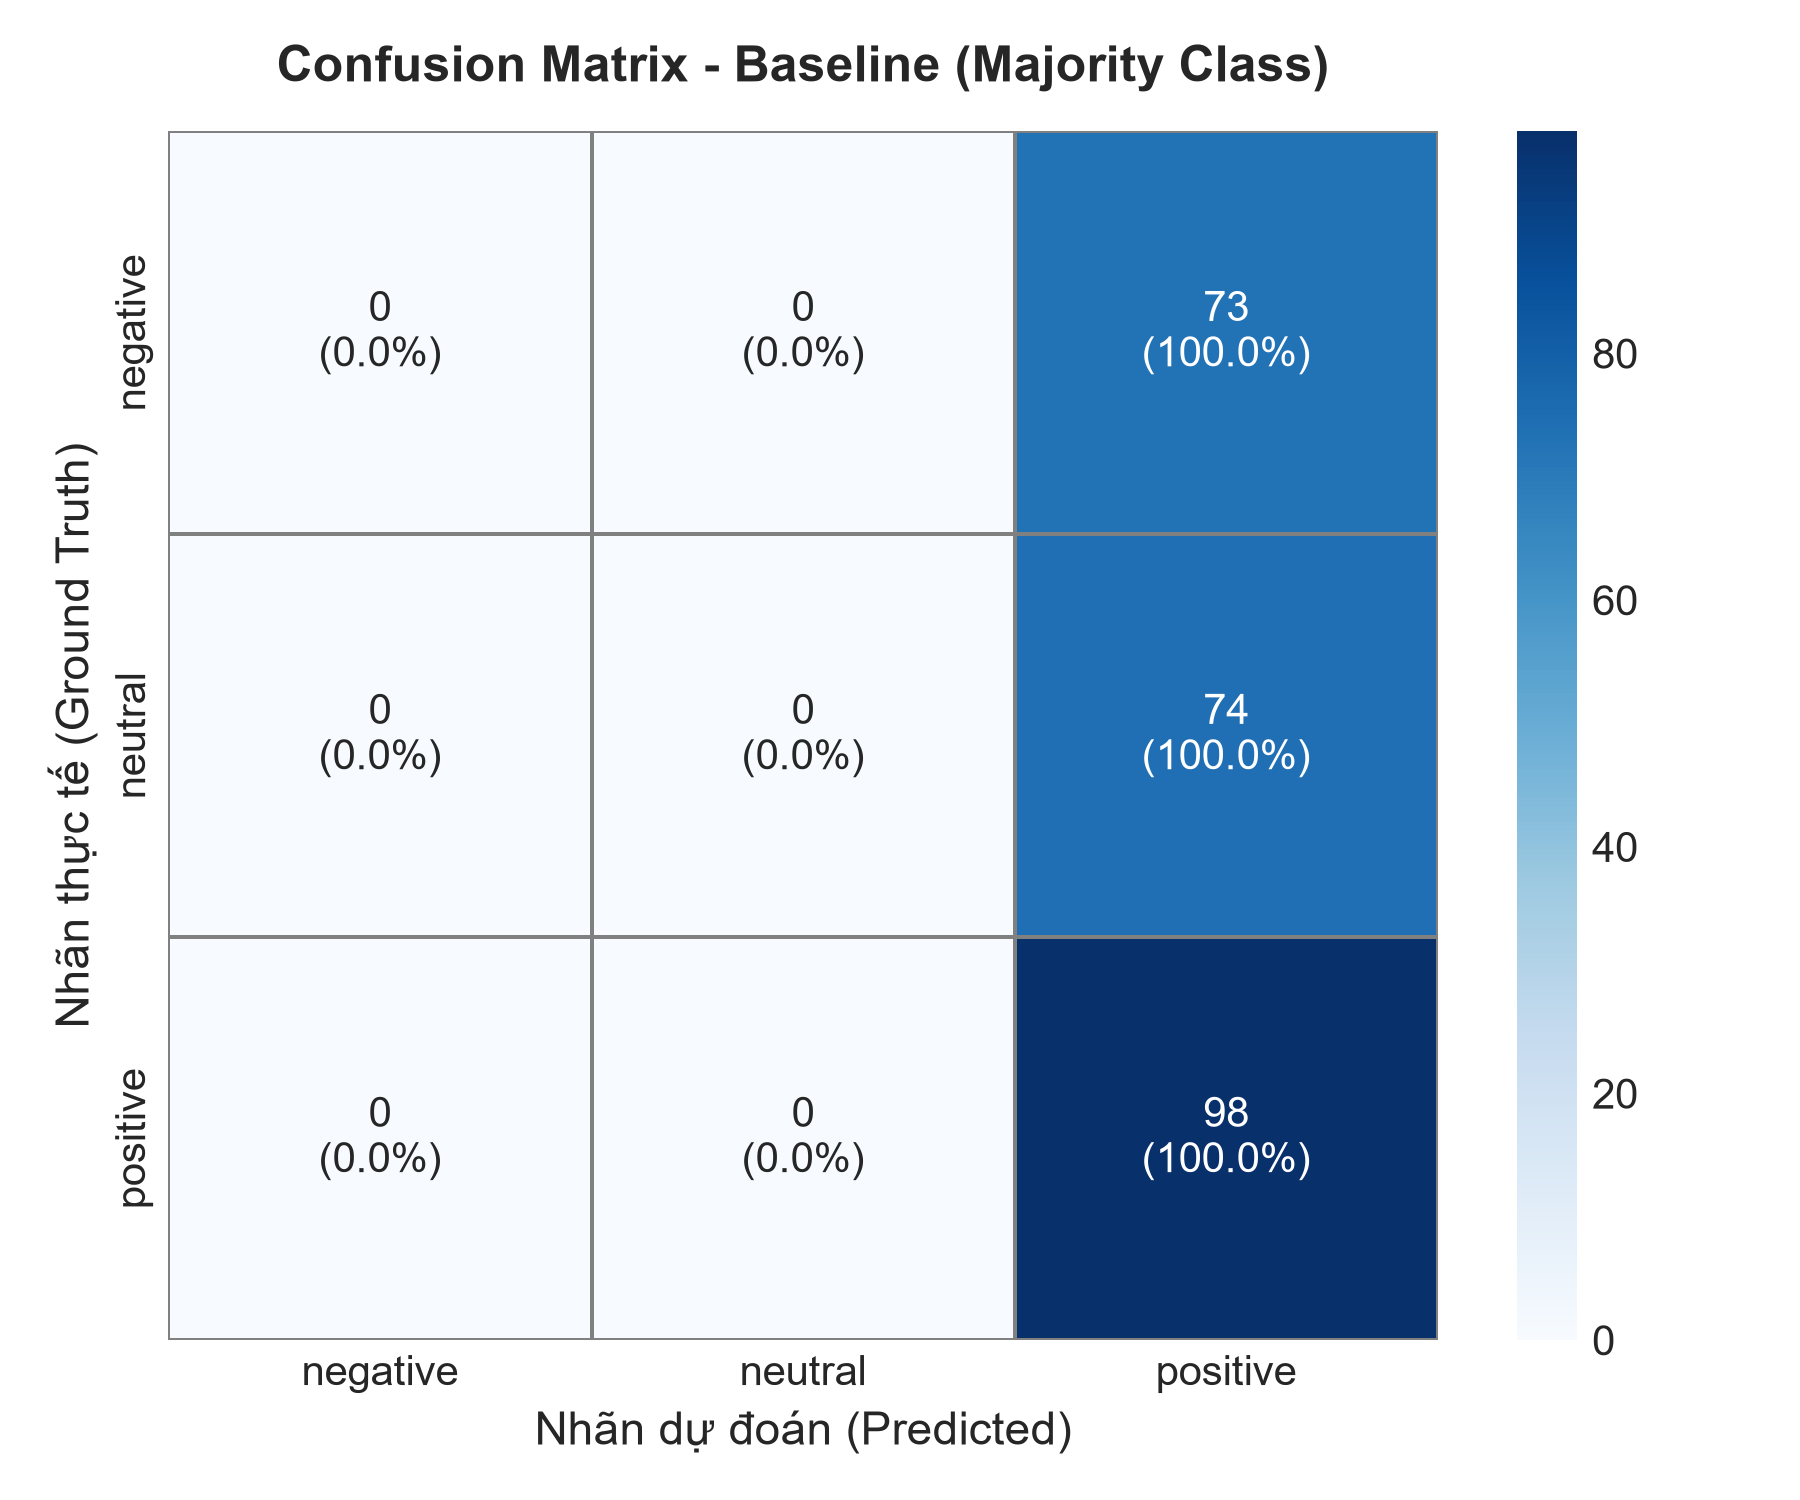
\includegraphics[width=\textwidth]{../figures/confusion_matrix_baseline.png}
        \caption{Baseline (Majority Class)}
    \end{subfigure}
    \hfill
    \begin{subfigure}[b]{0.48\textwidth}
        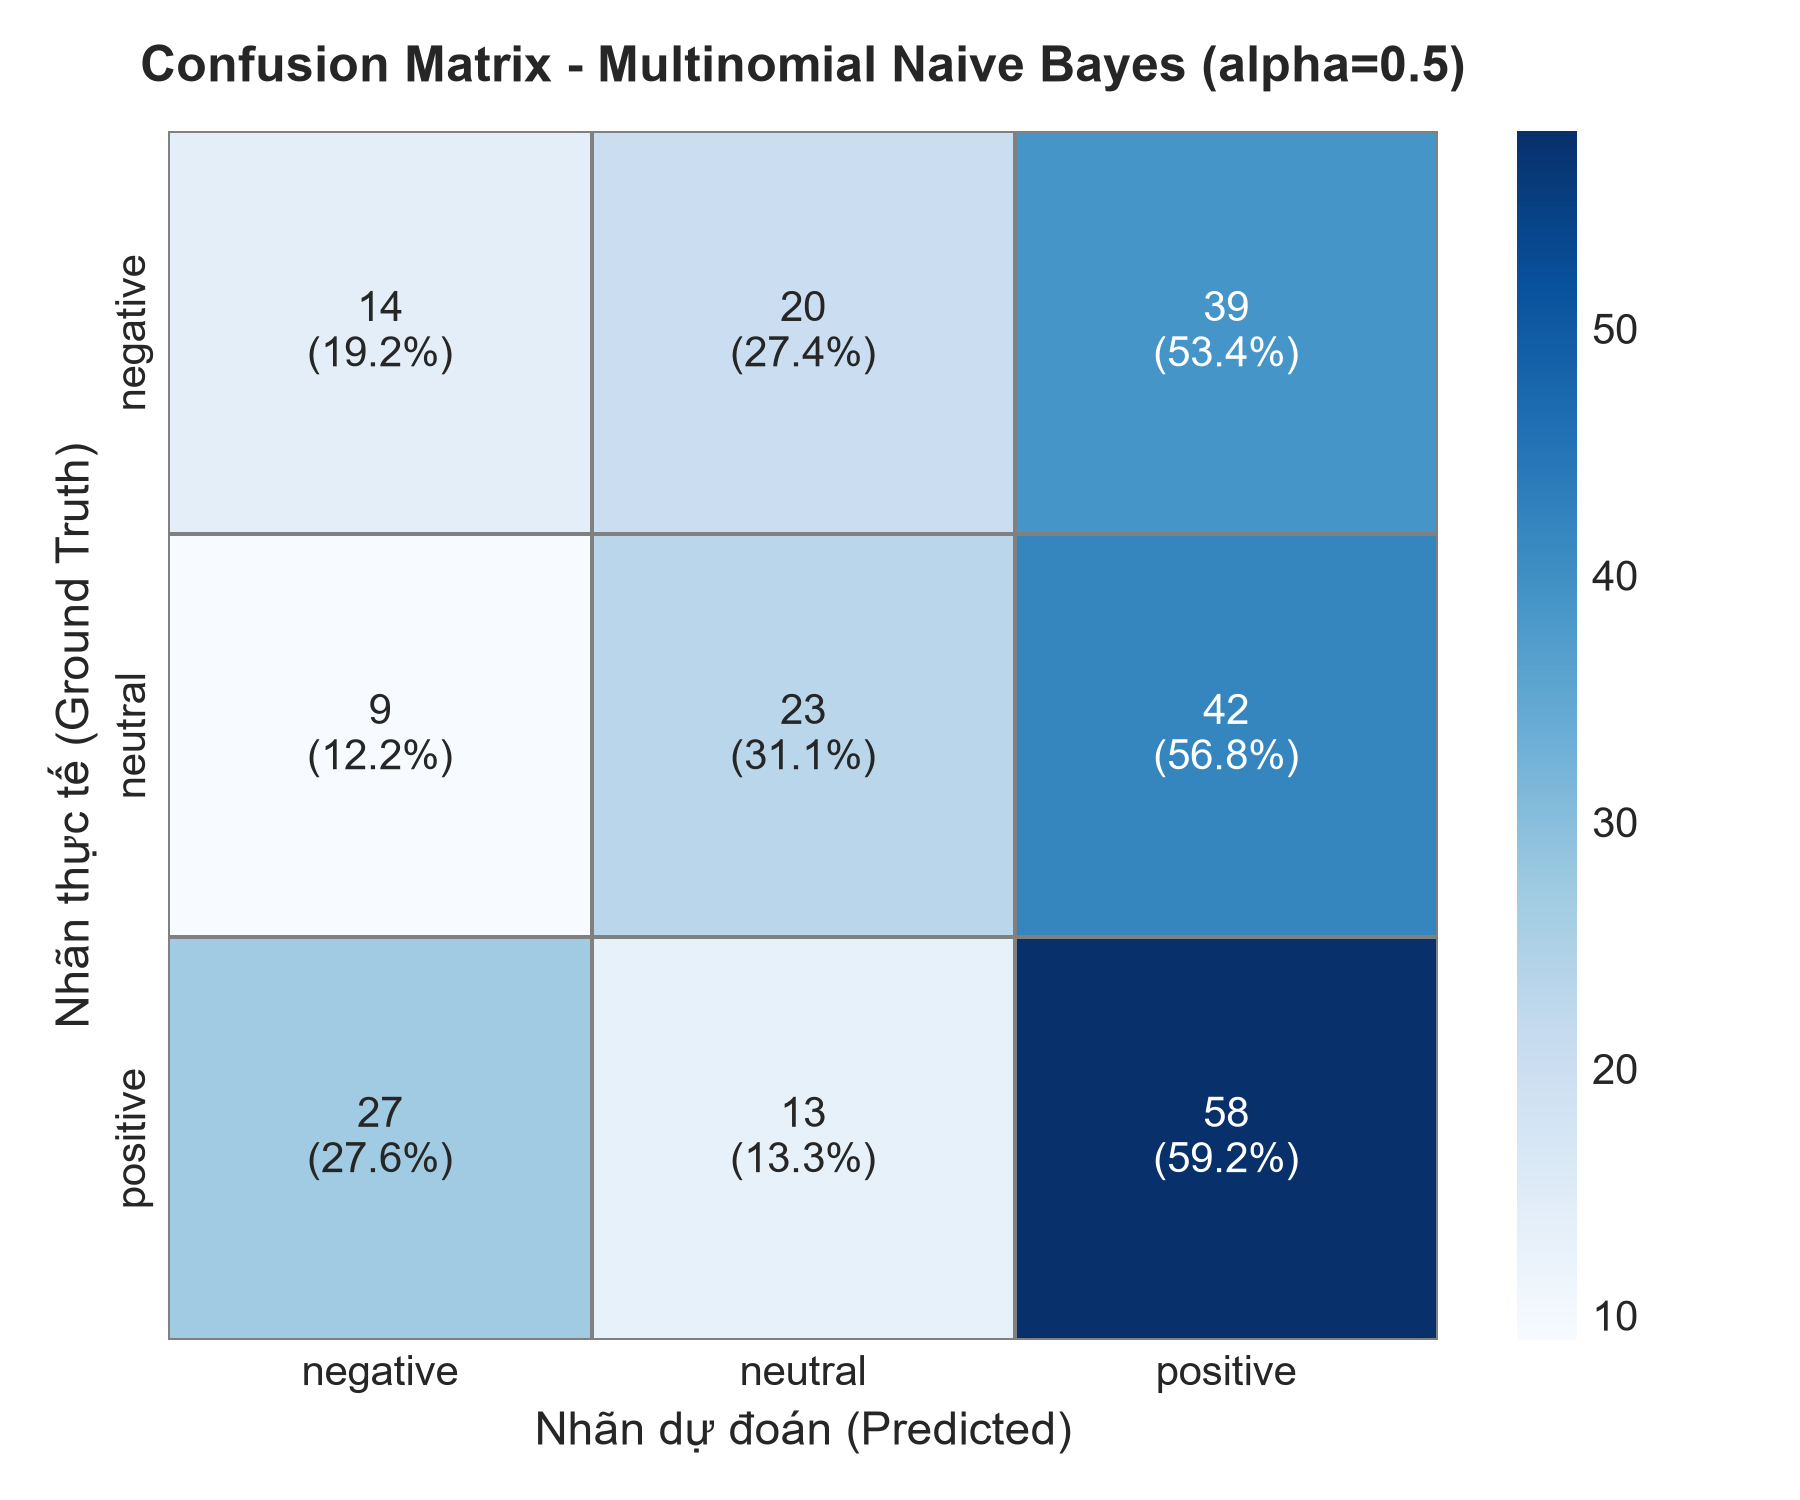
\includegraphics[width=\textwidth]{../figures/confusion_matrix_naive_bayes.png}
        \caption{Multinomial Naive Bayes ($\alpha=0.5$)}
    \end{subfigure}
    
    \vspace{0.4cm}
    \begin{subfigure}[b]{0.48\textwidth}
        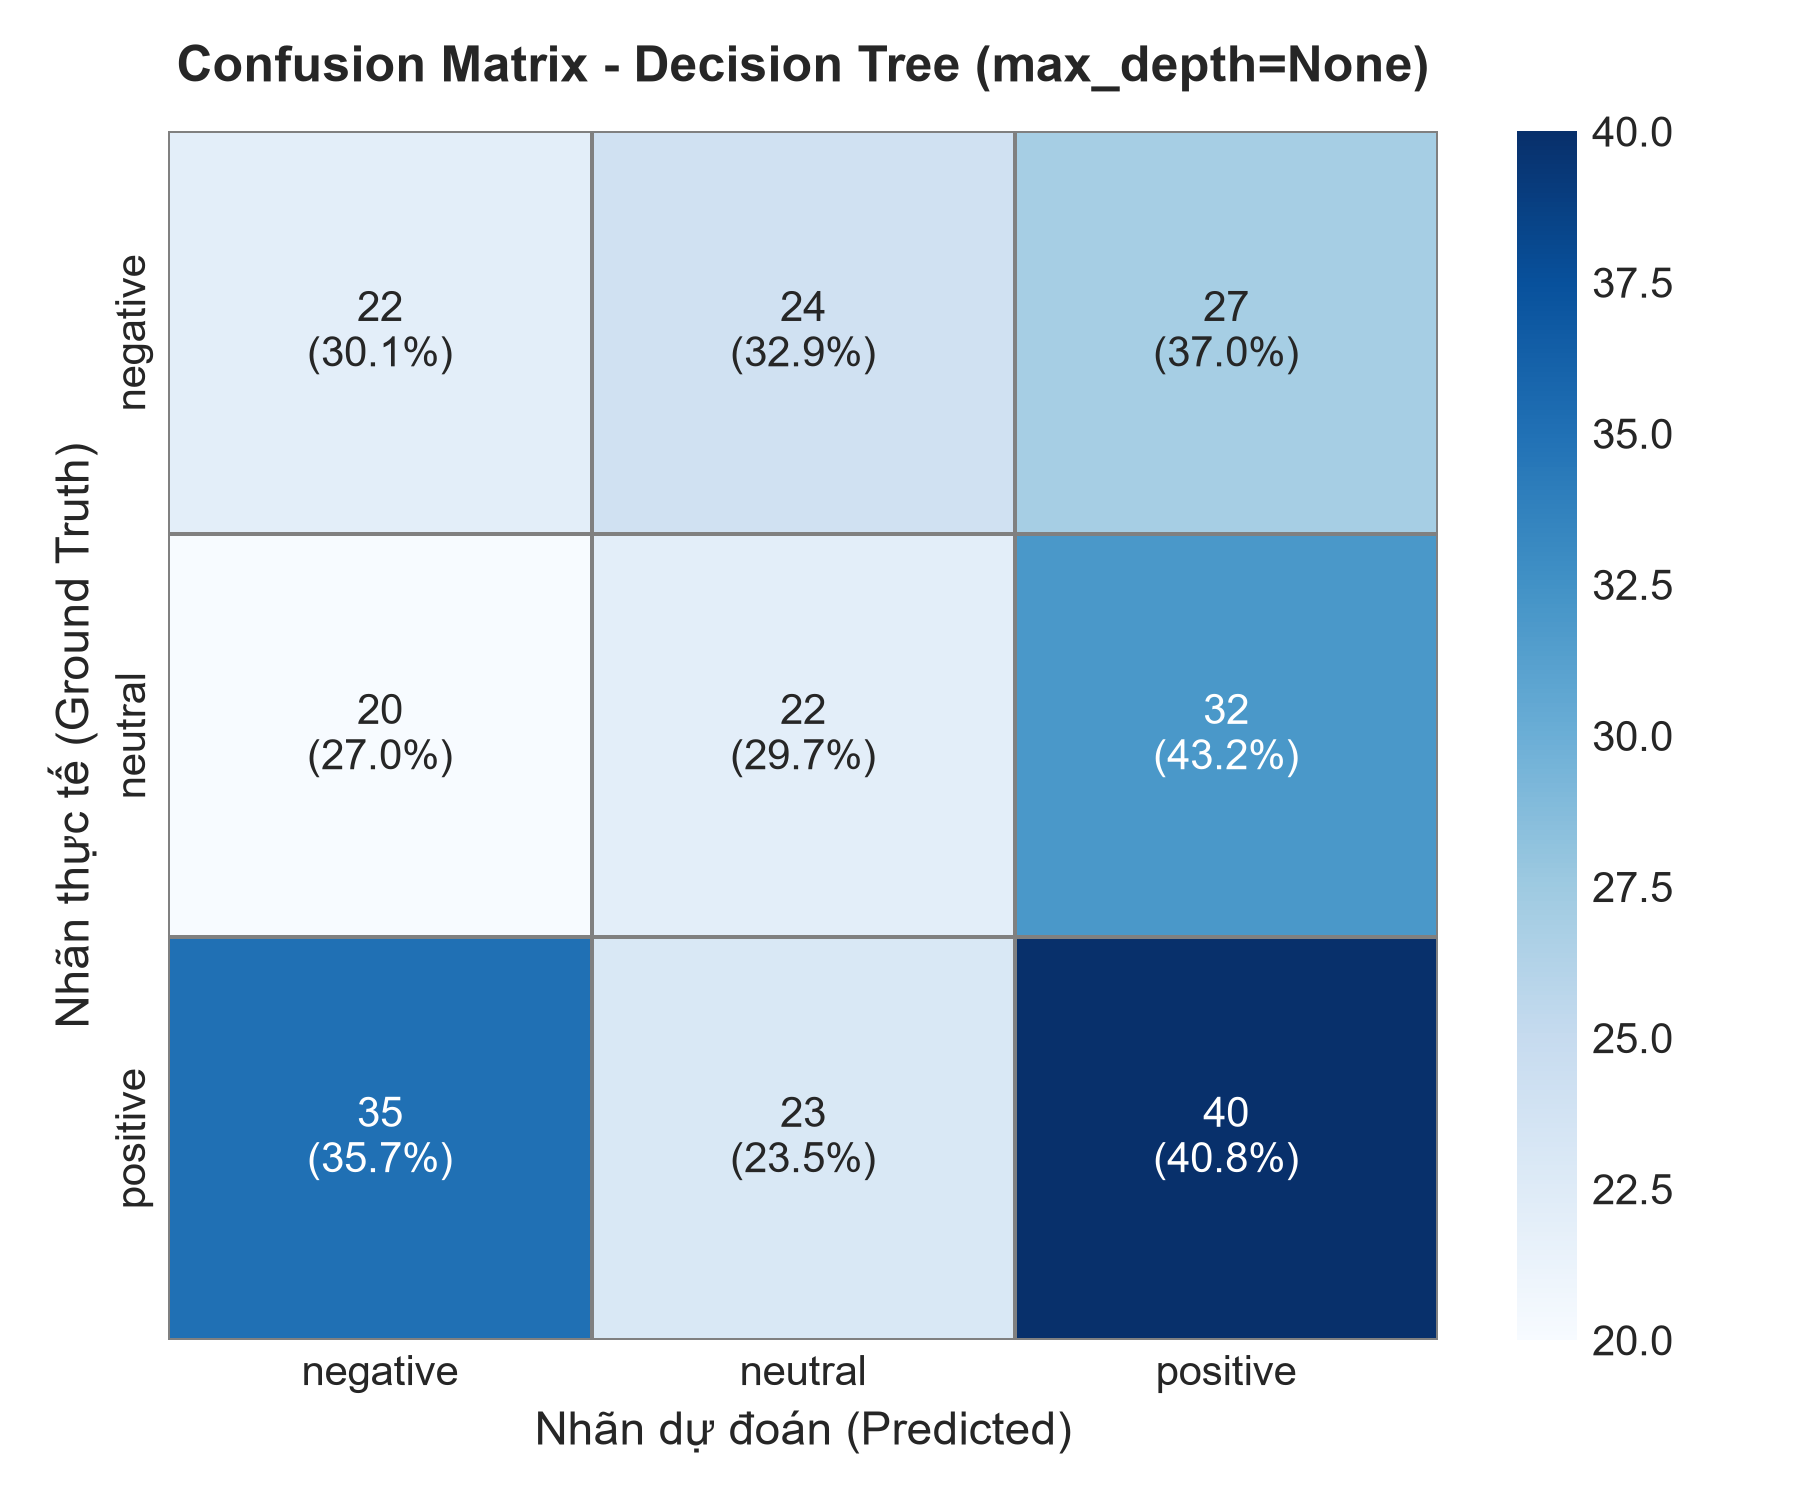
\includegraphics[width=\textwidth]{../figures/confusion_matrix_decision_tree.png}
        \caption{Decision Tree (\texttt{entropy})}
    \end{subfigure}
    \hfill
    \begin{subfigure}[b]{0.48\textwidth}
        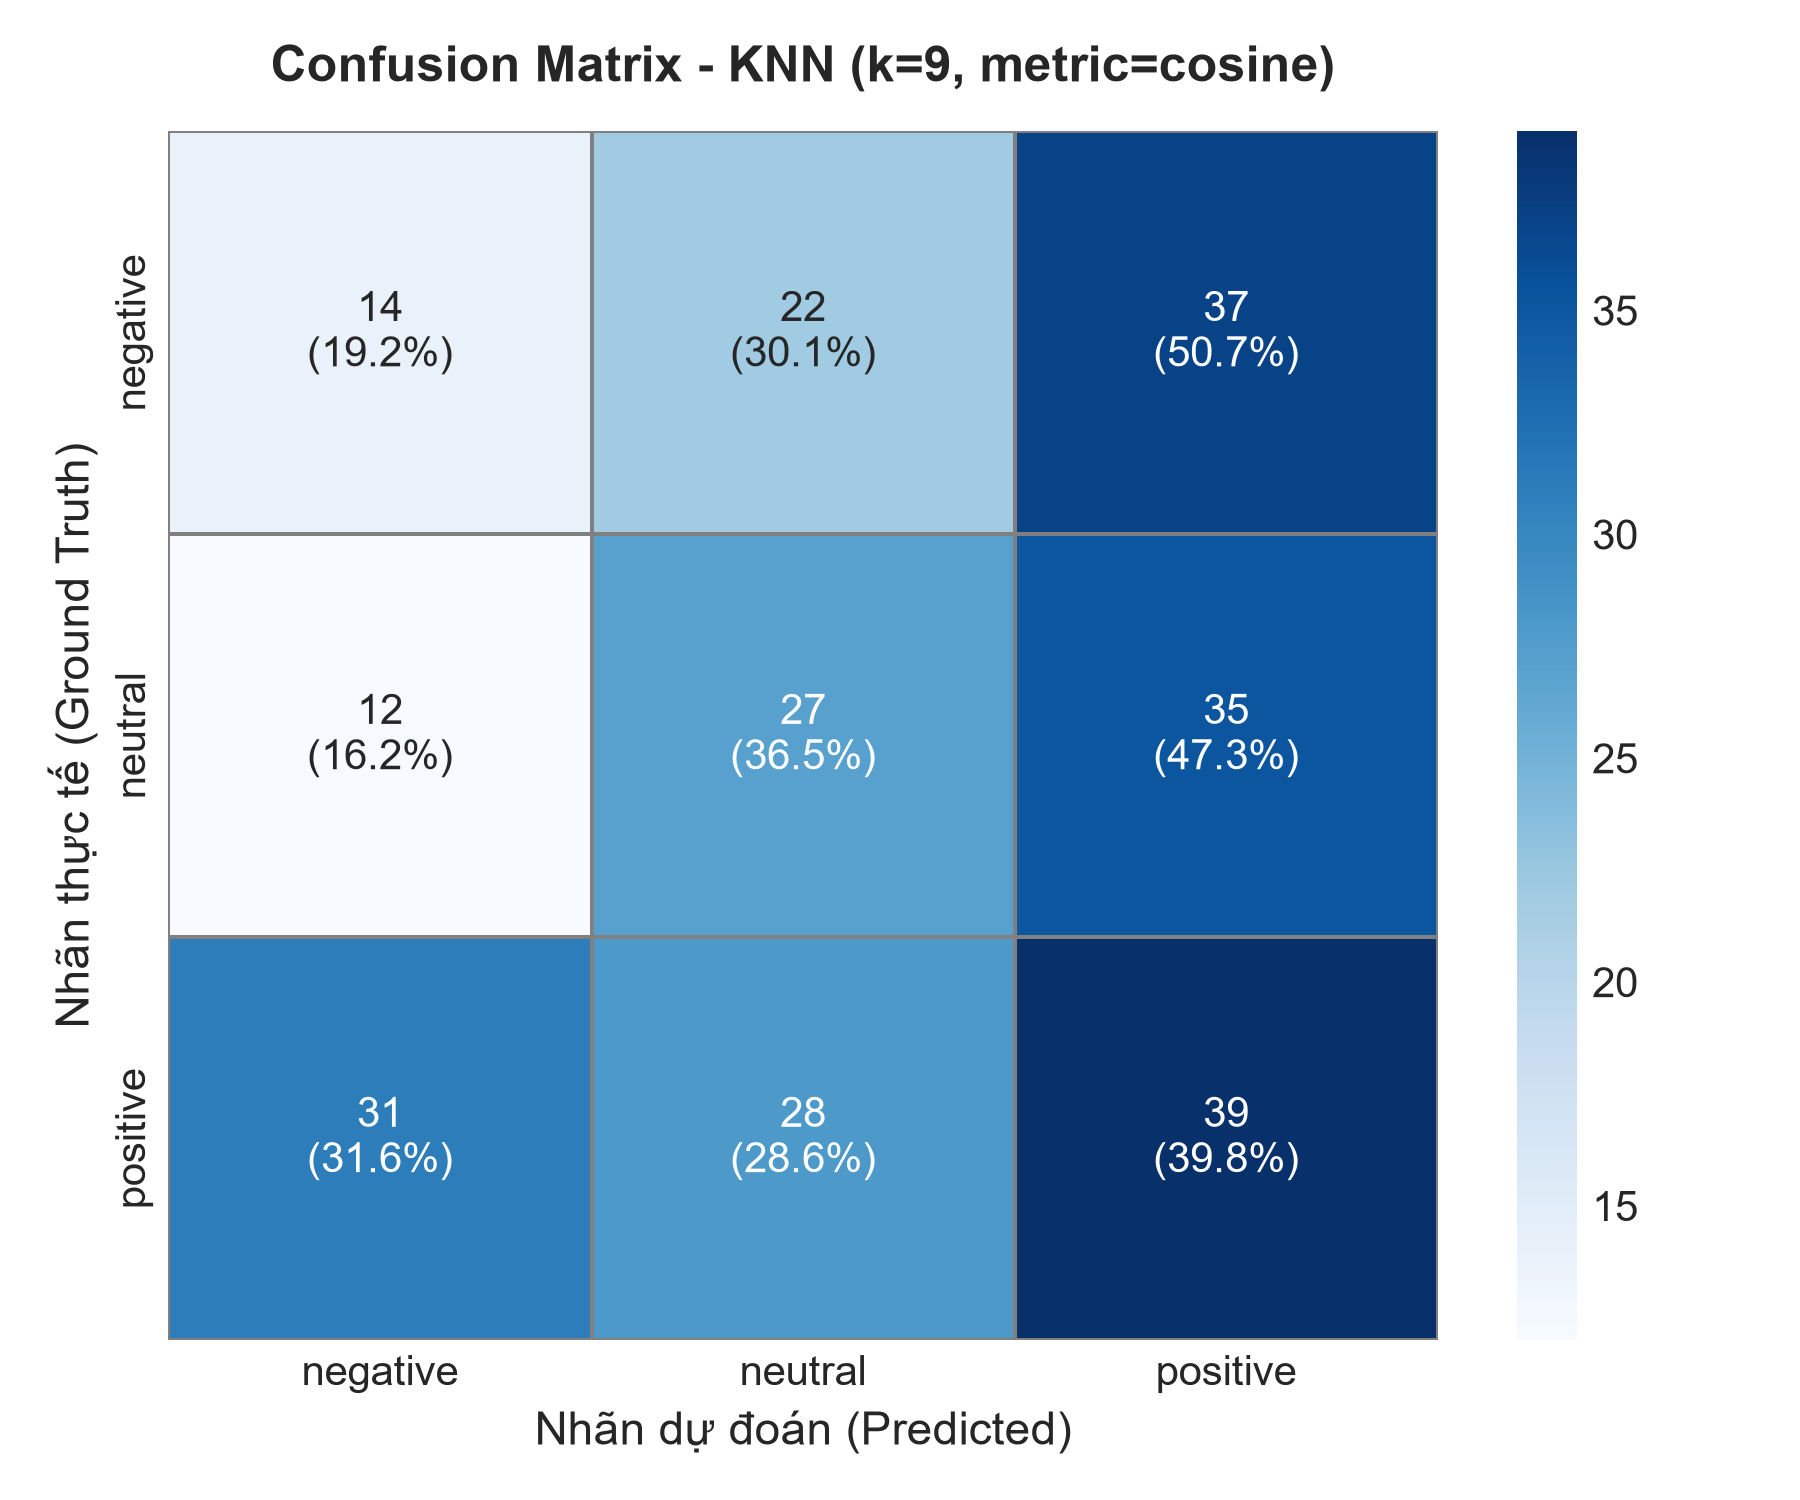
\includegraphics[width=\textwidth]{../figures/confusion_matrix_knn.png}
        \caption{K-Nearest Neighbors ($k=9$, cosine)}
    \end{subfigure}
    \caption{Ma trận nhầm lẫn (Confusion Matrix) của các mô hình trên tập kiểm thử.}
    \label{fig:cms}
\end{figure}

\newpage
\section{Thảo luận và so sánh}

\subsection{So sánh ưu nhược điểm của các phương pháp thử nghiệm}
\begin{itemize}
    \item \textbf{Về phương pháp biểu diễn đặc trưng:} 
    Kết quả thực nghiệm cho thấy việc đưa \textbf{Bigram} vào mô hình khiến Macro F1 sụt giảm nghiêm trọng (từ $0.3605$ xuống còn $0.2545$ trên TF-IDF). Nguyên nhân là do Bigram làm tăng kích thước từ điển từ $767$ lên tới $8,601$ đặc trưng (gấp hơn 11 lần). Với tập dữ liệu huấn luyện khiêm tốn ($978$ câu ngắn), đa số các cặp 2 từ chỉ xuất hiện đúng 1 lần duy nhất, dẫn đến ma trận đặc trưng cực kỳ thưa thớt, làm phân tán ước lượng xác suất của mô hình. Biểu diễn \textbf{Unigram} mang lại sự ổn định và khái quát hóa cao nhất.
    
    \item \textbf{Vì sao Multinomial Naive Bayes vượt trội hơn Decision Tree và KNN?}
    \begin{enumerate}
        \item \textbf{Naive Bayes:} Hoạt động dựa trên ước lượng xác suất độc lập có điều kiện. Do không cố gắng phân chia không gian đặc trưng phức tạp mà chỉ tính tích xác suất của các từ quan sát được, Naive Bayes có độ chệch (bias) nhất định nhưng phương sai (variance) rất thấp, cực kỳ bền vững trước dữ liệu thưa và nhiều chiều. Nhờ đó, MNB đạt Macro-F1 cao nhất ($0.3570$) và có độ cân bằng tốt giữa cả ba lớp.
        \item \textbf{Decision Tree:} Bản chất của Cây quyết định là phân chia trực giao không gian đặc trưng dựa trên từng thuộc tính đơn lẻ. Trong văn bản với hàng trăm từ vựng phân tán, việc phân nhánh theo sự có mặt của 1 từ cụ thể tại các tầng sâu nhanh chóng làm số mẫu tại các nút lá giảm xuống rất nhỏ, dẫn đến hiện tượng quá khớp (overfitting) nghiêm trọng trên tập train nhưng dự đoán kém trên tập test (Accuracy giảm xuống $34.29\%$).
        \item \textbf{K-Nearest Neighbors (KNN):} Bị ảnh hưởng nặng nề bởi "Lời nguyền số chiều" (Curse of Dimensionality). Trong không gian hàng trăm chiều với các vector thưa thớt, khoảng cách giữa các cặp điểm dữ liệu có xu hướng trở nên tương đương nhau, làm mờ nhạt khái niệm "láng giềng gần nhất", dẫn đến hiệu năng thấp nhất ($32.65\%$).
    \end{enumerate}
\end{itemize}

\subsection{Phân tích lỗi (Error Analysis)}
Thực hiện phân tích chi tiết trên $150$ mẫu dự đoán sai của mô hình tốt nhất (Multinomial Naive Bayes) trên tập kiểm thử (Bảng \ref{tab:error_pairs}):

\begin{table}[H]
\centering
\caption{Phân phối các cặp nhầm lẫn phổ biến nhất của Multinomial Naive Bayes}
\label{tab:error_pairs}
\begin{tabular}{llc}
\toprule
\textbf{Nhãn thực tế (Actual)} & \textbf{Nhãn dự đoán (Predicted)} & \textbf{Số lượng mẫu nhầm lẫn} \\
\midrule
Neutral & Positive & 42 \\
Negative & Positive & 39 \\
Positive & Negative & 27 \\
Negative & Neutral & 20 \\
Positive & Neutral & 13 \\
Neutral & Negative & 9 \\
\bottomrule
\end{tabular}
\end{table}

\textbf{1. Sự nhầm lẫn giữa nhãn Neutral và Positive/Negative:}
Có tới $42$ mẫu Neutral bị nhầm sang Positive và $20$ mẫu Negative bị nhầm sang Neutral. Các câu phản hồi trung tính thường mang tính chất nhận xét khách quan (ví dụ: mô tả thời khóa biểu, tài liệu môn học) nhưng lại chứa một số từ thường xuất hiện trong câu tích cực (như \textit{teacher, help, clear}). Do giả định độc lập túi từ không hiểu được cấu trúc ngữ pháp tổng thể, mô hình dễ bị nghiêng về nhãn chiếm ưu thế từ vựng.

\textbf{2. Tác động của yếu tố Châm biếm (Sarcasm):}
\begin{table}[H]
\centering
\caption{Tỷ lệ dự đoán sai theo cờ châm biếm (\texttt{sarcasm\_flag})}
\label{tab:sarcasm_err}
\begin{tabular}{lcc}
\toprule
\textbf{Nhóm dữ liệu} & \textbf{Tỷ lệ dự đoán sai (Error \%)} & \textbf{Tỷ lệ dự đoán đúng (Correct \%)} \\
\midrule
Không châm biếm (\texttt{sarcasm\_flag = 0}) & 59.41\% & 40.59\% \\
Có châm biếm (\texttt{sarcasm\_flag = 1}) & \textbf{69.77\%} & \textbf{30.23\%} \\
\bottomrule
\end{tabular}
\end{table}

Bảng \ref{tab:sarcasm_err} cung cấp bằng chứng định lượng rõ nét: Khi câu phản hồi mang tính chất châm biếm/mỉa mai, \textbf{tỷ lệ lỗi tăng vọt lên gần 70\%} (so với 59.4\% ở câu bình thường). Trong các câu châm biếm, sinh viên thường sử dụng các từ tích cực bề mặt (như "great", "wonderful", "love") để chỉ trích một vấn đề tiêu cực. Do mô hình túi từ chỉ đếm tần số từ độc lập mà không hiểu được hàm ý mỉa mai ngược nghĩa, mô hình tất yếu dự đoán sai.

\subsection{Hạn chế của bộ dữ liệu và giải pháp}
\begin{itemize}
    \item Bộ dữ liệu có quy mô khiêm tốn ($1,223$ mẫu) và văn bản phản hồi tương đối ngắn, khiến mật độ tín hiệu cảm xúc trên từng câu không đủ mạnh.
    \item Việc chỉ sử dụng văn bản đơn lẻ mà bỏ qua các trường siêu dữ liệu (metadata như khoa chuyên môn, phân loại phản hồi hay bối cảnh môn học) làm hạn chế nguồn thông tin bổ trợ quý giá.
\end{itemize}

\newpage
\section{Tổng kết và hướng phát triển}

\subsection{Tóm tắt kết quả chính}
\begin{enumerate}
    \item Báo cáo đã xây dựng thành công một quy trình học máy hoàn chỉnh, có tính tái lập cao cho bài toán phân loại cảm xúc phản hồi của sinh viên.
    \item Quy trình tiền xử lý và trích xuất đặc trưng được thực hiện đúng chuẩn học máy: bảo lưu các từ mang sắc thái phủ định quan trọng và kiểm soát hoàn toàn rủi ro rò rỉ dữ liệu (data leakage) giữa tập Train và tập Test.
    \item \textbf{Multinomial Naive Bayes} được chứng minh là thuật toán phù hợp và hiệu quả nhất trong số các thuật toán đã học đối với dữ liệu văn bản thưa thớt (Macro-F1 đạt 0.3570, vượt xa mô hình Baseline 0.1905).
    \item Phân tích thực nghiệm chỉ ra rõ các hạn chế cốt lõi của Cây quyết định và K-NN khi đối mặt với không gian đặc trưng văn bản nhiều chiều, cũng như tác động làm suy giảm hiệu năng của yếu tố châm biếm.
    \item Nhóm đã hoàn thành xuất sắc sản phẩm mở rộng: \textbf{Ứng dụng Web tương tác Demo (Streamlit)} hỗ trợ dự đoán trực tiếp và trực quan hóa phân phối xác suất.
\end{enumerate}

\subsection{Hướng phát triển trong tương lai}
\begin{itemize}
    \item \textbf{Tích hợp đa phương thức đặc trưng (Feature Fusion):} Kết hợp các đặc trưng văn bản (TF-IDF) cùng các thuộc tính dạng bảng sẵn có trong bộ dữ liệu (\texttt{department}, \texttt{feedback\_type}, \texttt{subject\_specific\_context}) qua các phương pháp mã hóa One-Hot hoặc Target Encoding.
    \item \textbf{Khai thác mô hình ngôn ngữ nâng cao:} Khi được mở rộng phạm vi môn học, nhóm đề xuất thử nghiệm các mô hình nhúng ngữ cảnh sâu (như Sentence-BERT hay RoBERTa tiếng Anh) để nắm bắt chính xác ngữ nghĩa của các câu có cấu trúc ngữ pháp phức tạp và câu châm biếm.
\end{itemize}

\newpage
\appendix
\section*{Phụ lục: Khai báo sử dụng AI và Liêm chính học thuật}
\addcontentsline{toc}{section}{Phụ lục: Khai báo sử dụng AI và Liêm chính học thuật}

Tuân thủ quy định tại Mục 2.3 và Mục 2.5 của tài liệu Hướng dẫn thực hiện bài tập lớn, nhóm sinh viên xin khai báo minh bạch việc sử dụng công cụ AI:
\begin{itemize}
    \item \textbf{Công cụ sử dụng:} Trợ lý AI Antigravity / Gemini của Google DeepMind.
    \item \textbf{Mục đích sử dụng:}
    \begin{itemize}
        \item Gợi ý tối ưu hóa biểu thức chính quy (Regex) trong bước tiền xử lý chuỗi văn bản.
        \item Hỗ trợ cấu hình cú pháp \texttt{GridSearchCV} của thư viện Scikit-Learn và các hàm vẽ biểu đồ Seaborn/Matplotlib.
        \item Hỗ trợ cấu trúc template soạn thảo báo cáo khoa học bằng mã nguồn \LaTeX.
    \end{itemize}
    \item \textbf{Cam kết của nhóm:} Toàn bộ số liệu thực nghiệm, kết quả huấn luyện mô hình, bảng đánh giá và phân tích lỗi đều được chạy thực tế 100\% trên máy tính cá nhân từ tập dữ liệu được chỉ định. Toàn bộ thành viên trong nhóm hiểu rõ quy trình toán học và mã nguồn của đề tài, cam kết bảo vệ độc lập và tự tin trả lời mọi câu hỏi vấn đáp của Giảng viên hướng dẫn.
\end{itemize}

\bibliographystyle{IEEEtran}
\bibliography{references}

\end{document}
